\documentclass[journal]{IEEEtran}
% \documentclass[5p,times,twocolumn]{elsarticle}
\usepackage{framed,multirow}
\usepackage{url}
\usepackage{xcolor}
\usepackage{hyperref}
\usepackage{amssymb}
\usepackage{latexsym}
\usepackage{amsmath,amsfonts}
\usepackage{booktabs}
\usepackage{subfigure}
\usepackage{xcolor}
\usepackage{amssymb}
\usepackage{adjustbox}
\usepackage{makecell}
\usepackage{hyperref}
\usepackage{graphicx}
\usepackage{tikz}


% \definecolor{darkgreen}{RGB}{0,150,0}
% \usepackage{pifont}
% \newcommand{\cmark}{\textcolor{darkgreen}{\ding{51}}}
% \newcommand{\xmark}{\textcolor{red}{\ding{55}}}
% \definecolor{LightRed}{rgb}{1,0.92,0.92}
% \definecolor{LightOrange}{rgb}{1,0.95,0.88}
% \definecolor{LightYellow}{rgb}{1.0,1.0,0.84}
% \definecolor{LightGreen}{rgb}{0.9,1.0,0.88}
% \definecolor{LightCyan}{rgb}{0.9,1,1}
% \definecolor{LightBlue}{rgb}{0.9,0.94,1}
% \definecolor{LightIndigo}{rgb}{0.92,0.9,1}
% \definecolor{LightMagenta}{rgb}{0.96,0.86,1}
% \definecolor{DirtyWhite}{rgb}{0.96,0.96,0.96}



\newcommand*{\jq}[1]{\textcolor{purple}{JQ: #1}}
\newcommand*{\mb}[1]{\textcolor{magenta}{MB: #1}}
\newcommand*{\aq}[1]{\textcolor{cyan}{AQ: #1}}

\begin{document}


%\title{Open Foundation Models \& LLMs in Healthcare: State of the Art, Challenges, and a Case Study on GenAI Driven Personalized Prescription} %Case Study} %Generative AI Based Prescription Case Study}

% \title{Open Foundation Models in Healthcare:\\ Challenges, Paradoxes, State of the Art, and a GenAI Driven Personalized Prescription Case Study} %Case Study} %Generative AI Based Prescription Case Study}

\title{Open Foundation Models in Healthcare: Challenges, Paradoxes, and Opportunities with GenAI Driven Personalized Prescription} %Case Study} %Generative AI Based Prescription Case Study}

\author{Mahdi Alkaeed$^{1}$, Sofiat Abioye$^{2}$, Adnan Qayyum$^{3}$, Yosra Magdi Mekki$^{4}$, Ilhem Berrou$^{5}$, Mohamad Abdallah$^{3}$,\\ Ala Al-Fuqaha$^{3}$, Muhammad Bilal$^{2}$, and Junaid Qadir$^{1}$ \\
$^1$Department of Computer Science and Engineering, College of Engineering, Qatar University, Doha, Qatar \\
$^2$Birmingham City University, Birmingham, United Kingdom \\
$^3$College of Science and Engineering, Hamad Bin Khalifa University (HBKU), Doha, Qatar \\
% $^3$Information Technology University (ITU), Lahore, Pakistan\\
$^4$College of Medicine, Qatar University, Doha, Qatar \\
$^5$University of the West of England (UWE), Bristol, United Kingdom\\
}

\maketitle

\begin{abstract}
In response to the success of proprietary Large Language Models (LLMs) such as OpenAI's GPT-4, there is a growing interest in developing open, non-proprietary LLMs and AI foundation models (AIFMs) for transparent use in academic, scientific, and non-commercial applications. Despite their inability to match the refined functionalities of their proprietary counterparts, open models hold immense potential to revolutionize healthcare applications. In this paper, we examine the prospects of open-source LLMs and AIFMs for developing healthcare applications and make two key contributions. Firstly, we present a comprehensive survey of the current state-of-the-art open-source healthcare LLMs and AIFMs and introduce a taxonomy of these open AIFMs, categorizing their utility across various healthcare tasks. Secondly, to evaluate the general-purpose applications of open LLMs in healthcare, we present a case study on personalized prescriptions. This task is particularly significant due to its critical role in delivering tailored, patient-specific medications that can greatly improve treatment outcomes. In addition, we compare the performance of open-source models with proprietary models in settings with and without Retrieval-Augmented Generation (RAG). Our findings suggest that, although less refined, open LLMs can achieve performance comparable to proprietary models when paired with grounding techniques such as RAG. Furthermore, to highlight the clinical significance of LLMs-empowered personalized prescriptions, we perform subjective assessment through an expert clinician. We also elaborate on ethical considerations and potential risks associated with the misuse of powerful LLMs and AIFMs, highlighting the need for a cautious and responsible implementation in healthcare.

\end{abstract}


\begin{IEEEkeywords}
AI Foundation Models (AIFMs), Large Language Models (LLMs), Retrieval-Augmented Generation (RAG), Personalized Prescriptions, and LLMs for Healthcare.
\end{IEEEkeywords}





\section{Introduction}
Recent years have witnessed an upsurge in the development of various \textbf{A}rtificial \textbf{I}ntelligence \textbf{F}oundation \textbf{M}odels (AIFMs) for different tasks such as Natural Language Processing (NLP), computer vision, healthcare, etc. This trend is primarily driven by the availability of extensive datasets and advancements in Deep Learning (DL) such as transformer networks. Notable milestones include attention networks (213 million parameters) \cite{wang2017heterogeneous}, GPT-2 (1.5 billion parameters) \cite{radford2019language}, GPT-3 (175 billion parameters) \cite{mann2020language}, the switch transformer (1.6 trillion parameters), Persia (100 trillion parameters) \cite{fedus2022switch}, and the recently unveiled GPT-4 (undisclosed parameters) \cite{bubeck2023sparks}. Specifically, scaling of model sizes has resulted in significant improvements in the performance of these AIFMs across classical NLP benchmarks such as GLUE \cite{wang2018glue}, SuperGLUE \cite{wang2018glue}, and Winograd \cite{sakaguchi2021winogrande}. Furthermore, AIFMs have shown their efficacy as few-shot learners \cite{brown2020language,wornow2024zero}, fueling their widespread adoption as foundational pre-trained models \cite{chen2020recall,chua2021fine,ju2022robust,vulic2021lexfit,zhang2020revisiting}.

Following the success of ChatGPT driven by proprietary Large Language Models (LLMs) like GPT-4 from OpenAI, there is increasing interest in open and nonproprietary LLMs. These models are positioned for broader community use in academic, scientific, and noncommercial endeavors. Although some open-source AI models have emerged, the landscape is in flux and the selection of models increasingly depends on performance, licensing, and integration capabilities. Although these open models often do not match the refined functionality of proprietary counterparts like GPT-4, they promise to revitalize healthcare applications when tailored to specific tasks. For example, open AIFMs can be repurposed to analyze vast medical literature, clinical guidelines, and patient data, thus helping healthcare professionals make more accurate diagnoses by considering a broader range of information and patterns than human capabilities, ultimately improving healthcare outcomes. Nevertheless, various lingering doubts and ethical considerations arise, particularly regarding the potential misuse of such powerful models for malicious purposes.  

This paper emphasizes the latest advancements and practical applications of open LLMs and AIFMs in healthcare. We evaluate the impact of open AI on healthcare and present the opportunities, capabilities, and challenges presented by current open AIFMs in this field. It is important to note that a concrete definition of open AI models is currently unavailable in the literature. Seger et al. \cite{seger2023open} defined open AI models as models for which the underlying training data, source code, and model weights are publicly available. On the other hand, Kapoor et al. \cite{kapoorposition} followed a reductive approach to define open AI models as models with widely available weights. In addition, the security, robustness, and privacy of these models remain unaddressed, as these models are not as polished as proprietary closed-source models and trail behind the current capabilities of proprietary closed-source LLMs and AIFMs \cite{thieme2023foundation,seger2023open}.

\textit{Contributions of the Paper:} To the best of our knowledge, this article is the first comprehensive survey focused on open AIFM and LLM for healthcare care and presents a promising case study on the use of these models for the critical clinical prescription task. The following are the salient contributions of this paper:

\begin{enumerate}
    \item We present a comprehensive survey on open-source LLMs and AIFMs in healthcare, providing readers with information on the latest advances in this domain.
    \item We present a taxonomy of open AIFMs for different healthcare applications including medical imaging, clinical NLP, medical education, diagnosis, etc.
    \item We present a case study utilizing the general purpose (open-source) LLMs for prescription and adverse risk assessment tasks. Specifically, we present an empirical analysis of various open-source LLMs including LLaMA-2, LLaMA-3, Mistral, and Meditron, and compare their performance with a famous proprietary model, i.e., Open AI's GPT4. Also, we investigate how integrating Retrieval-Augmented Generation (RAG) can enhance the performance of open-source LLMs in this critical clinical task. 
\end{enumerate}

\textit{Organization of the Paper:}
The remaining paper is structured as follows: Section \ref{sec:back} provides an overview of the relevant background related to open-source LLMs and AIFMs and their associated challenges. Section \ref{sec:sota_review} provides an overview of the existing state-of-the-art literature on open LLMs and AIFMs in the healthcare domain. Section \ref{sec:case_study} presents the methodology and results of our case study on personalized prescriptions. Finally, we conclude the paper in Section \ref{sec:concs}. 

% The organization of the paper is shown in Figure \ref{Fig:OrgnaizationofPaper}.

\section{Background}
\label{sec:back}

\subsection{LLMs and AI Foundation Models: A Brief Overview}
LLMs represent the recent advancements in large general models characterized by their immense size and capacity to perform various NLP tasks including understanding and generating human-like text \cite{vaswani2017attention}. LLMs are typically pre-trained on large datasets containing vast amounts of text from the Internet. During pre-training, the model learns to predict the next word in a sentence or fill in missing parts of text. This unsupervised pre-training allows the model to capture contextual information and syntactic structures. After pre-training, LLMs can be fine-tuned on specific tasks with smaller datasets. Fine-tuning adapts the model to perform tasks such as text classification, language translation, summarization, etc. These models can generate coherent and contextually relevant text given a prompt. LLMs have been used for various downstream tasks such as creative writing, code generation, question answering, and different natural language understanding tasks \cite{he2023survey}. The success of LLMs in solving various NLP tasks has attracted substantial attention from the research community and has resulted in the development of AIFMs, which are also referred to as general-purpose AI models. These models possess general capabilities that can be tailored to model a variety of downstream tasks, including healthcare applications. In healthcare, LLMs can be used for tasks such as medical record summarization, patient data analysis, diagnostic assistance, and personalized treatment recommendations, showcasing their potential to enhance patient care and streamline medical processes significantly \cite{bommasani2021opportunities}.

% One of the prime examples of open LLMs is LLaMA-2 and LLaMA-3, which currently allow user interactions using prompts. 

\begin{figure*} [!t]
\centering
\includegraphics[width=\linewidth]{openness_level.png}
\caption{\textbf{Levels of Open-Source Access for LLMs and AIFMs.} The figure shows the spectrum from Fully Closed Source to Fully Open Source, detailing key aspects and descriptions for each level. (Adapted from \cite{solaiman2023gradient}).}
\label{fig:openness}
\end{figure*}

\subsection{Open Source LLMs and AI Foundation Models}
In recent years, several open AI models have emerged, yet the landscape remains dynamic and the model selection is increasingly dependent on their performance, licensing, and integration capabilities \cite{roziere2023code}. However, these open models often fall short of the refined functionality of proprietary models such as GPT-4. The concept of Open AI or open source AI remains nebulous, frequently embodying aspirations or marketing tactics rather than a concrete definition \cite{seger2023open}. These terms reflect the principles of free and open-source software (FOSS), emphasizing the freedom to use, study, modify, and share software. Open LLMs and AIFMs extend this philosophy to AI, highlighting the importance of transparency, accessibility, and collaborative enhancement of these models. The decision between open-source and closed-source models involves balancing the freedom for customization against proprietary features and commercial support offered by closed-source models. Open LLMs and AIFMs are distributed under various licenses \cite{carugati2023competition}, from the permissive MIT or Apache 2.0 (which allows considerable user freedom) to the more restrictive GNU General Public License (GPL) \cite{gurrieri2023d2}, which mandates that derivative works remain open-source. These licenses facilitate commercial use, modification, and distribution, while also imposing stipulations regarding copyright and patent rights. In the ML research and development community, doubts remain about the merits and drawbacks of making LLMs and AIFMs open-source or retaining them as proprietary models \cite{alizadeh2023open,seger2023open}.



% For an in-depth discussion on the implications of open-sourcing AI foundation models, refer to Nandita Jaya's article, "Foundation models: To open-source or not to open-source?"   Nevertheless, the openness of current “Open AI” tools has been contested; for instance, Meta's LLaMA-2 has faced criticism over the extent of its 'openness,' with concerns that big tech companies still exert considerable control (as discussed in "The Myth of Open-Source AI" at wired.com). Further examination of the political economy of Open AI is presented in a paper available at papers.ssrn.com.

\subsubsection{Requirements for Open LLMs and AIFMs}
The term open-source stems from the traditional Open-Source Software (OSS) context, defined in 1998 \cite{osi1998definition}. OSS requires software to be publicly available for use, viewing, modifications, and distributing source code under open-source license \cite{seger2023open, dibona1999open}. However, within the context of LLMs and AIFMs, the term ``open AI'' has become ambiguous. The degree of openness in existing open AI tools has been a subject of considerable debate. For example, LLaMA has encountered criticism regarding the extent of their openness \cite{touvron2023LLaMA}. For instance, Meta recently announced an open-source LLaMA-2 model; however, it has not been made available under a traditional open-source license. Instead, Meta has defined its terms and conditions regarding the use of this model for various IoT applications, especially in healthcare domains. In Figure \ref{fig:openness}, we present a gradient depicting the level of open-source access to LLMs and AIFMs, followed by a brief discussion of the pros and cons of open-sourcing these models.

The requirements for open AI are certainly different and various definitions are found in the relevant literature. For example, Seger et al. \cite{seger2023open} outlined the critical components of open-source AI models, encompassing everything from training data to the model itself. In contrast, Kapoor et al. \cite{kapoor2024societal} argued that open access to model weights alone suffices to classify a model as open AI. However, several components are involved in developing AI models, including model architecture, training data, hyperparameters, model weights, and documentation. Each of these components contributes to the overall transparency and functionality of the models. In common practice, developers often have the flexibility to choose which components of the open AI models they make public, which allows them to tailor their open-source approach based on the specific considerations of their project, taking into account factors such as proprietary concerns, collaboration preferences, and the nature of the AI application being developed. However, in the context of LLMs and AIFMs, the crucial open-source requirement is to provide open access to their weights. Therefore, merely releasing only one component of the models, such as the source code, does not qualify as a genuinely open-source model. There are various prospects for using open AI models in the healthcare domain, including enhancing medical research, improving diagnostic tools, and facilitating personalized treatment plans. For instance, open-source models could analyze large datasets of medical literature to identify new treatment protocols or assist clinicians by providing evidence-based recommendations tailored to individual patient needs.  


% \begin{figure*} [!t]
% \centering
% \includegraphics[width=0.95\linewidth]{OpenLLMs_AIFMs2.png}
% \caption{\textbf{Key Components of Open LLMs and AIFMs for Healthcare}. This diagram highlights the six essential components: Model Architecture, Model Weights, Inference Code, Training Code, Training Data, and Licensing.}
% \label{fig:OpenLLMs_AIFMs}
% \end{figure*}


\subsubsection{Pros and Cons of Using Open AIFMs}
The recent work by Seger et al. \cite{seger2023open} describes the key advantages of using open LLMs and AIFMs across three dimensions including: 

\begin{enumerate}
    \item \textit{External Evaluation:} Open-sourcing LLMs and AIFMs provide an opportunity for the wider AI community to perform external audits and extensive evaluations on the AI system to identify its vulnerabilities to enhance the overall safety and robustness of models.
    \item  \textit{Acceleration in AI Progress:} Open-sourcing these models can drive significant advancements through collective and widespread collaboration among AI developers and researchers \cite{spector2023accelerating}.
    \item \textit{Distributed Control:} Open-sourcing LLMs and AIFMs can decentralize AI development, allowing smaller organizations to contribute. This approach democratizes AI but poses potential dangers such as risks regarding the misuse of these powerful models \cite{seger2023open}.
\end{enumerate}

In a recent study, Kapoor et al. \cite{kapoor2024societal} provided a comprehensive evaluation of the societal impact of open AIFMs. They identified five distinctive properties of these models: broader access, greater customizability, the potential for local inference, the inability to rescind model access once released, and weaker monitoring of the models' downstream use. The authors highlighted five significant benefits of open AIFMs: distributing decision-making power, reducing market concentration, increasing innovation, accelerating science, and enabling transparency. They emphasized how broader access and greater customizability facilitate innovation, allowing these models to be aggressively tailored to support various applications and advance the state-of-the-art across different languages. Furthermore, Kapoor et al. \cite{kapoor2024societal} introduced the concept of ``marginal risk'', which refers to the extent to which these models increase societal risk through intentional misuse compared to existing closed AIFMs or other technologies like web search. They also highlighted the challenge of enforcing restrictions on downstream usage in open-source models, noting that the open release of model weights is irreversible.

\subsection{Challenges Hindering Open AI in Healthcare}
\subsubsection{Data and Model Privacy}
In the literature, it has been argued that ensuring the privacy of patient data is a top priority \cite{khalid2023privacy}. AIFMs are typically trained on vast amounts of medical records, which may include sensitive, confidential, or personally identifiable information. Therefore, during the training process, the model can inadvertently memorize and reproduce this information when generating text, leading to data leakage \cite{inan2021training}. This can be a severe breach of privacy if the generated content is shared publicly or accessed by unauthorized/malicious entities. These extracted instances encompass publicly accessible personally identifiable information like names, phone numbers, and email addresses, along with medical records. Larger models tend to exhibit greater vulnerability compared to smaller ones \cite{carlini2021extracting,inan2021training}. Proper encryption, access controls, and compliance with healthcare regulations are essential to protect patient information \cite{torkzadehmahani2022privacy}. Training healthcare AIFMs necessitates access to large quantities of high-dimensional data, often derived from unfiltered user-generated content. This approach introduces substantial privacy risks \cite{carlini2021extracting, inan2021training, zou2020privacy, pan2020privacy, goldstein2023generative, bender2021dangers}.

\subsubsection{Model Security}
Researchers have demonstrated that AI models used in medical imaging can be vulnerable to adversarial attacks. For instance, the behaviors of an AI diagnosis model under adversarial images generated by Generative Adversarial Network (GAN) models could lead AI models to misdiagnose conditions such as cancer. This type of attack could potentially lead to incorrect treatment plans, posing severe risks to patient health \cite{zhou2021machine}. Various adversarial ML attacks can be realized on DL models that can be broadly categorized into two classes \cite{qayyum2020secure}: (1) targeted attacks, where the objective is to enforce the model to classify a given input into the target class; (2) untargeted attacks, where the objective is to increase overall misclassification rate. The enormity of these attacks has already been demonstrated for various ML-empowered medical systems such as medical image classification \cite{finlayson2018adversarial,finlayson2019adversarial,paschali2018generalizability}, abnormal heartbeat detection (i.e., ECG classification) \cite{han2020deep}, etc. Although open-sourcing AI models will expedite research in critical directions such as evaluating their security aspects, a cautious approach should be considered while openly releasing models trained using patient's sensitive data.  


\begin{figure*}[!h]
\centering
\includegraphics[width=\linewidth]{image_new.png}
%{ApplicationsOfLLMs.png}
\caption{\textbf{Applications of LLMs in Healthcare.} This figure shows six key areas: Clinical Documentation, Disease Prediction and Diagnosis, Drug Discovery, Virtual Health Assistants, NLP in EHRs, and Telemedicine Support.}
\label{fig:ApplicationsOfLLMs}
\end{figure*}

\subsubsection{Ethical Issues}
Healthcare applications are essentially human-centric and require careful consideration of ethical aspects throughout the development of AI-based medical systems. Therefore, it is imperative to understand the sociological needs of the targeted users before starting data collection for the development of the AI model. In addition, the ethical dimensions of AI applications in healthcare involve addressing biases, ensuring fairness, and contemplating the broader implications of AI-generated decisions on patient care \cite{wang2023ethical}. John et al. \cite{john2024re} argued that ethical debates need to be localized within the complex interplay of technical, legal, and organizational entities from which machine learning moral issues arise.

\subsubsection{Regulatory Issues}
The true transformative potential of AI can only be realized when these systems are integrated into clinical workflows; however, this is not a non-trivial task. Since the healthcare sector operates under stringent regulatory frameworks, such as the Health Insurance Portability and Accountability Act (HIPAA) \cite{oakley2023hipaa} and the General Data Protection Regulation (GDPR) \cite{carmi2023european}. Therefore, integrating AI solutions while adhering to these regulatory requirements demands careful navigation. The literature argues that the existing regulatory guidelines are insufficient for regulating AI-based medical systems, as these systems are adaptable (i.e., having an ever-evolving nature) and involve learning from new patient data \cite{qayyum2020secure}.    


\section{State-of-the-Art in Open Healthcare LLMs and AIFMs}
\label{sec:sota_review}

\subsection{Applications of LLMs and AIFMs in Healthcare}
The advent of LLMs has facilitated the investigation of their capabilities in the medical domain, enabling comprehension and communication through language. This development holds the promise of more immersive human-AI interaction and collaboration. Notably, these models have showcased remarkable proficiency in addressing multiple-choice research benchmarks \cite{wei2022chain,singhal2022large}. Moreover, multi-modal foundational models can learn visual features based on textual descriptions and can be adept at various tasks such as medical imaging analysis, disease detection in radiology, pathology slide interpretation, etc. Leveraging state-of-the-art architectures like convolutional neural networks (CNNs) and transformer-based models such CLIP \cite{radford2021learning}, language vision models can enhance diagnostic accuracy, streamline medical imaging workflows, and contribute to the development of advanced healthcare technologies such as VisionFM \cite{qiu2023visionfm}, RETFound \cite{zhou2023foundation}, and LVM-Med \cite{mh2024lvm}. Figure \ref{fig:ApplicationsOfLLMs} illustrates a spectrum of applications for LLMs within the healthcare domain. 

%This presentation highlights the multifaceted contributions of language models, illustrating their impact on various facets of healthcare.

Moreover, multi-modal LLMs can analyze and process data from various resources or modalities that include text (language), images (vision), and audio. The idea is to create such models that can understand and generate insights by jointly considering information from different types of data (such as Gloria \cite{lehmann2023gloria}, LLaVA \cite{yin2023lamm}, PLIP \cite{zuo2023plip}, etc.). The applications of LLMs in healthcare have emerged as a transformative force in the medical landscape. LLMs and AIFMs offer a versatile set of applications that significantly impact various facets of healthcare. From automating clinical documentation to early disease prediction, for instance, LLMs such as BERT \cite{praveen2023understanding}, BioBERT \cite{sharaf2023analysis}, and ChatGPT \cite{vaishya2023chatgpt} have demonstrated their prowess in efficiently processing complex medical information. In addition, these models can be leveraged for drug discovery, personalized medicine, and literature review automation, showcasing their potential to accelerate research and enhance patient care. The integration of LLMs and multi-modal AIFMs into healthcare practices underscores their capacity to respond to diverse requests, making them valuable assets in advancing information processing and decision-making \cite{clusmann2023future}. 



\subsubsection{Applications in Tabular Data Analysis}
LLMs offer a diverse range of applications, including automating clinical documentation for enhanced accuracy and extracting structured data from unstructured EHR information \cite{wornow2023shaky}. It also facilitates streamlining coding and billing processes, providing real-time insights for clinical decision support, improving information search through NLP, facilitating population health management through trend analysis, enabling voice-to-text transcription for efficient record updates, enhancing patient engagement with personalized summaries, ensuring data quality through automated quality assurance, and supporting healthcare research with advanced analytics. The integration of LLMs into EHRs thus plays a pivotal role in optimizing healthcare workflows, enhancing decision-making, and ultimately improving patient outcomes \cite{wang2023anypredict,guo2023ehr}.

\subsubsection{Applications in Clinical NLP}
Various NLP techniques are used to extract structured information from EHRs, converting free-text data into a format that can be easily analyzed for research, decision support, and other healthcare applications. Clinical NLP applications are diverse and impactful in healthcare \cite{singhal2023large}. They include improving clinical documentation accuracy, extracting structured information from EHRs, aiding clinical decision support, extracting phenotypic information for research, detecting adverse drug events, expediting clinical trial recruitment, understanding temporal relationships in patient records, de-identifying data for privacy compliance, and facilitating voice-to-text transcription in clinical settings. Powerful LLMs like ChatGPT (GPT-4) demonstrate significant potential for processing text data within the medical domain through zero-shot in-context learning \cite{liu2023deid,waisberg2023gpt,ali2023chatgpt,ali2023chatgpt}. Clinical notes exhibit significant differences from biomedical literature, leading to subpar performance of BERT models pre-trained on clinical notes, similar to the standard BERT model \cite{gu2021domain}.

\subsubsection{Applications in Prognosis, Diagnosis, and Medicine}
LLMs play a crucial role in healthcare across different applications, including prognosis, diagnosis, and medicine \cite{sun2023pathasst,balas2023conversational}. In the prognosis task, they aid in outcome prediction and disease progression modeling. Similarly, LLMs can provide automated diagnostic support \cite{levine2023diagnostic}, analyze medical images for abnormalities, and assist in identifying rare diseases. In medicine, LLMs can be leveraged for drug discovery, enable personalized treatment plans, and help monitor and improve medication adherence \cite{xie2023faithful,biswas2023chatgpt,wornow2024zero}.

\subsubsection{Applications in Medical Imaging}
In addition to LLMs that particularly work for different NLP tasks, the advancements in vision foundation models such as Segment Anything (SAM) have significant potential to revitalize medical image analysis \cite{deng2023segment}. These models, often built on DL architectures, are trained to analyze and interpret various types of medical images, such as X-rays \cite{putz2023segment}, MRIs \cite{zhao2023clinical}, CT scans \cite{chen2023pancreatic}, and pathology slides, for instance, Med-PaLM \cite{singhal2023large}, a prompt-tuned iteration of Flan-PaLM 540B \cite{nori2023capabilities}. These models can be used for various applications, including medical image classification, segmentation, disease diagnostics, and detection of abnormalities \cite{li2023artificial}. The integration of large vision models should consider combining information from these diverse modalities to extract complementary features, thereby enhancing diagnostic accuracy \cite{zhang2023challenges,shi2023generalist,ji2304segment}.

% \begin{figure*} [!t]
% \centering
% \includegraphics[width=0.95\linewidth]{TimelineLLMs.png}
% \caption{\textbf{Timeline of LLMs in Healthcare (2021-2024).} This figure shows the progression of LLMs in healthcare, highlighting the development of increasingly capable (and multimodal) models each year from 2021 to 2024.}
% \label{fig:TimelineLLMs}
% \end{figure*}

\subsubsection{Applications in Healthcare Delivery}
LLMs can significantly enhance healthcare delivery by streamlining patient communication by generating clear materials and powering telemedicine platforms \cite{dash2023evaluation}. For instance, the literature demonstrates that they can improve operational efficiency by automating administrative tasks and supporting clinical decision-making for dental medicine \cite{eggmann2023implications}. LLMs play a key role in quality improvement, health education, and remote patient monitoring, fostering proactive interventions \cite{vaishya2023chatgpt}. Moreover, LLMs can address language barriers, facilitate care coordination, and collectively contribute to a more effective and patient-centered healthcare delivery.

\subsubsection{Applications in Medical Education}
LLMs significantly contribute to the evolution of medical education \cite{eysenbach2023role,kung2023performance}. LLMs have numerous applications in medical education, for instance, they can facilitate curriculum development, generate varied educational content \cite{van2023if}, support global accessibility through language translation \cite{fraiwan2023review}, assist in assessment and evaluation with adaptive tools \cite{abd2023large}. Furthermore, LLMs and AIFMs-empowered simulators can enable lifelike clinical case simulations, empowering interactive e-learning platforms \cite{teebagy2023improved}, contributing to continuing medical education \cite{antaki2023evaluating}, facilitating summarization of intricate medical literature \cite{gill2023chatgpt}. Also, LLMs have the potential to significantly impact and transform psychological health assessment education \cite{kjell2023ai}. These applications improve the efficiency, accessibility, and personalization of medical education, meeting the dynamic requirements of students and professionals in the healthcare sector \cite{li2023chatgpt,ray2023chatgpt}. In practical terms, the Chatdoctor \cite{yunxiang2023chatdoctor} and other LLMs could be designed to assist users with medical queries, provide information about symptoms, offer general health advice, or even engage in conversation about medical topics \cite{li2023chatdoctor,wu2023pmc,haupt2023ai,javaid2023chatgpt,johnson2023assessing,moons2023chatgpt}. Moreover, ChatGPT can be used to disseminate accurate and up-to-date medical information to users, serving as an educational tool to provide information about symptoms, diseases, medications, and general health advice \cite{iftikhar2023docgpt,ide2023can,muftic2023exploring,de2023chatgpt}.


\subsubsection{Applications in Telehealth}
LLMs offer various potential applications in telehealth that can significantly enhance the delivery and accessibility of healthcare services. For instance, LLM-based virtual assistance and chatbots can provide patients with timely information and support. Similarly, LLMs can enable healthcare providers to efficiently assess patient conditions and prioritize care based on urgency. In addition, LLMs can streamline appointment scheduling and send automated reminders, thereby improving patient compliance and reducing no-show rates. They also play a critical role in patient health monitoring and reporting, enabling continuous assessment of health metrics and timely intervention when necessary. Furthermore, LLMs can assist in remote follow-ups, providing patients with essential information regarding their treatment plans and recovery processes. The integration of LLMs in telehealth not only enhances the efficiency of healthcare delivery but also contributes to improved patient outcomes by ensuring that individuals receive personalized and timely care \cite{snoswell2023artificial}.

\subsubsection{Applications in Surgical Science}
AI models, including CCNs, such as Flan-PaLM  \cite{singhal2023large}, can be employed for image recognition in surgical procedures. They help identify and analyze structures and anomalies in surgical frames, aiding surgeons in diagnostics and preoperative planning. AI plays a crucial role in robot-assisted surgery, where robotic systems are guided by intelligent algorithms \cite{ahmed2024deep}. These systems can enhance precision, minimize invasiveness, and provide real-time feedback to surgeons during procedures. AI algorithms can predict when surgical equipment might require maintenance or calibration \cite{nori2023can}. The literature highlights that such a proactive approach ensures that surgical tools are in optimal condition during procedures \cite{abi2023large}. 

% Figure \ref{fig:TimelineLLMs} illustrates the timeline of existing open LLMs in recent years in healthcare domains.

% \begin{table*}[!h]
%     \centering
% \scriptsize
%     \caption{Summary for existing open LLMs developed for various healthcare applications. Legend: FC: fully closed source; HA: hosted access, API: access to the model is provided through the cloud; MR: model is publicly released; CR: code for the model training is released; D: model documentation is released; and FOS: fully open source.
%     }
%     \begin{tabular}{ p{1.45cm} p{5 cm} p{4.5cm} p{3.3cm} p{0.7cm} p{0.7cm} }
%     \toprule
%      \textbf{Model Name}  & \textbf{Description} 
%      & \textbf{Performance Achievements} & \textbf{Application/Domain } & \textbf{Code} & \textbf{Level} \\ \toprule
%     BioBERT (2020) \cite{lee2020biobert} & Domain-specific language representation model pre-trained on extensive biomedical corpora. & Maintains nearly identical architecture across various tasks. & Biomedical Text Mining & \href{https://huggingface.co/pritamdeka/BioBERT-mnli-snli-scinli-scitail-mednli-stsb}{Link} & 
%     APIs
%     \\
%     \midrule
%     BioMegatron (2020) \cite{shin2020biomegatron} & Model for efficient model parallel training of LLMs with 8.3 billion parameters. & Trained from scratch on a comprehensive domain corpus from PubMed. & Biomedical Text Representation & \href{https://huggingface.co/EMBO/BioMegatron345mUncased}{Link} &
%     CR
%     \\
%     \midrule
%     Med-BERT (2021) \cite{rasmy2021med} & Contextualized embedding model pre-trained on a structured EHR dataset. & Demonstrates substantial enhancements in prediction accuracy. & EHRs, Disease Prediction & \href{https://huggingface.co/trueto/medbert-kd-chinese}{Link} & 
%     APIs
%     \\
%     \midrule
%     BioELECTRA (2021) \cite{raj2021bioelectra} & Specialized language encoder model for the biomedical domain, adapted from ELECTRA. & Pre-trained on PubMed and PMC full-text articles. & Biomedical Text Representation & \href{https://huggingface.co/menadsa/S-BioELECTRA}{Link} & 
%     APIs
%     \\
%     \midrule
%     KeBioLM (2021) \cite{yuan2021improving} & Biomedical pre-trained language model using UMLS knowledge bases. & Outperformed other Pre-trained Language Models (PLMs) on Named Entity Recognition (NER) and Relation Extraction (RE). & Biomedical Text Mining, Named Entity Recognition, Relation Extraction & \href{https://github.com/GanjinZero/KeBioLM}{Link} 
%     &
%     CR
%     \\
%     \midrule
%     BioBART (2022) \cite{lu2022clinicalt5} & Specialized generative language model for biomedical applications, pre-trained on PubMed abstracts. & Exhibits improved performance in various tasks, including dialogue, summarization, and entity linking. & Dialogue, Summarization, Entity Linking & \href{https://huggingface.co/GanjinZero/biobart-v2-base}{Link} & 
%     MR
%     \\
%     \midrule
%     LinkBERT (2022) \cite{yasunaga2022linkbert} & Language model pretraining approach capitalizing on document links, surpasses BERT in performance across diverse downstream tasks. & Pre-trained on Wikipedia and PubMed with citation links. & General Domain, Biomedical Domain & \href{https://huggingface.co/michiyasunaga/LinkBERT-large}{Link} & 
%     APIs
%     \\
%     \midrule
%     BioGPT (2022) \cite{luo2022biogpt} & Domain-specific generative Transformer language model pre-trained on extensive biomedical literature corpus. & Evaluated across six biomedical NLP tasks. & Biomedical Natural Language Processing & \href{https://huggingface.co/microsoft/biogpt}{Link} 
%     &
%     APIs
%     \\
%     \midrule
%     RadBERT (2022) \cite{yan2022radbert} & BERT-based language models specifically tailored for radiology, pre-trained on millions of radiology reports. & Radiology, Medical Imaging & Pre-trained on U.S. Department of Veterans Affairs reports, six variants created & \href{https://huggingface.co/UCSD-VA-health/RadBERT-RoBERTa-4m}{Link} 
%     &
%     APIs
%     \\
%     \midrule
%     FastFold (2022) \cite{cheng2022fastfold} & Streamlined implementation of AlphaFold for both training and inference, introduces AutoChunk to decrease memory costs during inference. & Protein Folding, Structural Biology & Achieves over 80\% reduction in memory costs during inference, AutoChunk strategy & \href{https://github.com/hpcaitech/fastfold}{Link} 
%     &
%     D
%     \\
%     \midrule
%     Clinical BERT (2023) \cite{yang2023enhancing} & Designed for clinical notes and biomedical texts, trained on MIMIC-III. & Fine-tuned for clinical tasks like named entity recognition and question answering. 340 million parameters. & Clinical notes and biomedical texts. & \href{https://github.com/kexinhuang12345/clinicalBERT}{Link} 
%     &
%     FOS
%     \\
%     \midrule
%     LLaMA-2 (2023) \cite{touvron2023LLaMA} & A revised iteration of LLaMA-1, now trained on a novel blend of publicly accessible data. Additionally, the pretraining corpus size has been expanded by 40\%. & Tailored for dialogue scenarios. & Clinical Text Processing, Information Retrieval, text-to-text framework & \href{https://huggingface.co/meta-LLaMA/LLaMA-2-7b-chat-hf}{Link} 
%     &
%     MR
%     \\
%     \midrule
%     ChatDoctor (2023) \cite{wang2023chatcad} & A healthcare chat model refined through the application of medical domain expertise, using the LLaMA model as a foundation. & ChatDoctor excels in providing precise responses to patient queries by retrieving dependable information. & Medical Analysis, answer queries & \href{https://huggingface.co/zl111/ChatDoctor?text=Hey+my+name+is+Thomas%21+How+are+you%3F}{Link} 
%     &
%     MR
%     \\
%     \midrule
%     CPLLM (2023) \cite{shoham2023cpllm} & Clinical Prediction with Large Language Models (CPLLM) fine-tunes LLMs using prompts customized for medical concept sequences. & Utilizes ICD-9-CM and ICD-10-CM diagnoses datasets. & Clinical Prediction, Diagnosis Codes & \href{https://github.com/nadavlab/CPLLM}{Link} 
%     &
%     CR
%     \\
%     \midrule
%     DoctorGLM (2023) \cite{xiong2023doctorglm} & Trained on CMD data, fine-tuned using ChatGLM-6B model. & Processes approximately 80,000 Q and A pairs per hour per GPU. & Clinical Question-Answering & \href{https://github.com/xionghonglin/DoctorGLM}{Link} 
%     &
%     CR
%     \\
%     \midrule
%     Med-PaLM2 (2023) \cite{singhal2023towards} & Recently developed medical Language Model (LLM) trained with PaLM 2. & Achieved the first ``passing'' score in US Medical Licensing Examination-style questions, scoring 67.2\% on the MedQA dataset. & Medical Licensing Examination, Question Answering & \href{https://github.com/conceptofmind/PaLM}{Link} 
%     &
%     CR
%     \\
%     \midrule
    
%     GhatCAD (2024)
    
%     \cite{yang2022gatortron} & The Reliable Report Generation module can interpret medical images from various fields and produce high-quality medical reports & Enhanced consistency and reliability for interpretation and advice & Diagnosis on medical image & \href{https://github.com/zhaozh10/ChatCAD}{Link} & 
%     CR
%     \\
%     \midrule
    
%     HuatuoGPT-II (2024) \cite{zhang2023huatuogpt} & LLM tailored for medical consultations, combines data from ChatGPT with real-world data from doctors during supervised fine-tuning. & Medical Consultations, Natural Language Processing & Incorporates real-world data from doctors, emulates the performance of medical professionals & \href{https://github.com/FreedomIntelligence/HuatuoGPT}{Link} 
%     &
%     CR
%     \\
%     \midrule
%      DragonFly-Med (2024) \cite{chen2024dragonfly}
%      &
%      A new LMM architecture that improves detailed visual comprehension and reasoning about specific image regions.
%      & 
%      Handle high-resolution images, fine-tuned Dragonfly with biomedical instructions
%      & 
%      Visual commonsense reasoning and analyzing biomedical images
%      & \href{https://huggingface.co/togethercomputer/LLaMA-3-8B-Dragonfly-Med-v1}{Link}
%      &
%      MR
%      \\
%     \midrule
     
%      Merlin (2024) \cite{blankemeier2024merlin}
     
%      &
%      Trained to interpret 3D abdominal CT scans using supervision from structured EHRs.
%      & 
%       Zero-shot classification of findings, phenotype identification, zero-shot cross-modal retrieval
%      &
%      3D computed tomography.
%      & 
%      Soon
%      &
%      -
%     \\
%     \midrule
    
%      Meta Fair (2024)\cite{team2024chameleon}
     
%      &
%      Meta Chameleon is a family of models designed to handle both text and images as inputs and outputs. These models use a single unified architecture, enabling them to process and generate any combination of text and images.
%      & 
%      Capable of understanding and generating images and text in any arbitrary sequence using a single unified architecture for both encoding and decoding.
%      & 
%      Multimodel for both text and images
%      & 
%     \href{https://ai.meta.com/blog/meta-fair-research-new-releases/}{Link}
%      &
%      APIs
%     \\

 
%     \bottomrule 
%     \end{tabular}
%     \label{tab:OpenAI-models}
% \end{table*}

\begin{table*}[!t]
    \centering
    \scriptsize
    \caption{Summary of existing open LLMs developed for various healthcare applications. Legend: FC: fully closed source; HA: hosted access; API: access to the model is provided through the cloud; MR: model is publicly released; CR: code for the model training is released; D: model documentation is released; and FOS: fully open source.}
    \begin{tabular}{ p{1.45cm} p{5 cm} p{4.5cm} p{3.3cm} p{0.7cm} p{0.7cm} }
    \toprule
    \textbf{Model Name}  & \textbf{Description} & \textbf{Performance Achievements} & \textbf{Application/Domain} & \textbf{Code} & \textbf{Level} \\ 
    \midrule
    BioBERT (2020) \cite{lee2020biobert} & Domain-specific language representation model pre-trained on extensive biomedical corpora. & Maintains nearly identical architecture across various tasks. & Biomedical Text Mining & \href{https://huggingface.co/pritamdeka/BioBERT-mnli-snli-scinli-scitail-mednli-stsb}{Link} & APIs \\ 
    \midrule
    BioMegatron (2020) \cite{shin2020biomegatron} & Model for efficient model parallel training of LLMs with 8.3 billion parameters. & Trained from scratch on a comprehensive domain corpus from PubMed. & Biomedical Text Representation & \href{https://huggingface.co/EMBO/BioMegatron345mUncased}{Link} & CR \\ 
    \midrule
    Med-BERT (2021) \cite{rasmy2021med} & Contextualized embedding model pre-trained on a structured EHR dataset. & Demonstrates substantial enhancements in prediction accuracy. & EHRs, Disease Prediction & \href{https://huggingface.co/trueto/medbert-kd-chinese}{Link} & APIs \\ 
    \midrule
    BioELECTRA (2021) \cite{raj2021bioelectra} & Specialized language encoder model for the biomedical domain, adapted from ELECTRA. & Pre-trained on PubMed and PMC full-text articles. & Biomedical Text Representation & \href{https://huggingface.co/menadsa/S-BioELECTRA}{Link} & APIs \\ 
    \midrule
    KeBioLM (2021) \cite{yuan2021improving} & Biomedical pre-trained language model using UMLS knowledge bases. & Outperformed other Pre-trained Language Models (PLMs) on Named Entity Recognition (NER) and Relation Extraction (RE). & Biomedical Text Mining, Named Entity Recognition, Relation Extraction & \href{https://github.com/GanjinZero/KeBioLM}{Link} & CR \\ 
    \midrule
    BioBART (2022) \cite{lu2022clinicalt5} & Specialized generative language model for biomedical applications, pre-trained on PubMed abstracts. & Exhibits improved performance in various tasks, including dialogue, summarization, and entity linking. & Dialogue, Summarization, Entity Linking & \href{https://huggingface.co/GanjinZero/biobart-v2-base}{Link} & MR \\ 
    \midrule
    LinkBERT (2022) \cite{yasunaga2022linkbert} & Language model pretraining approach capitalizing on document links, surpasses BERT in performance across diverse downstream tasks. & Pre-trained on Wikipedia and PubMed with citation links. & General Domain, Biomedical Domain & \href{https://huggingface.co/michiyasunaga/LinkBERT-large}{Link} & APIs \\ 
    \midrule
    BioGPT (2022) \cite{luo2022biogpt} & Domain-specific generative Transformer language model pre-trained on extensive biomedical literature corpus. & Evaluated across six biomedical NLP tasks. & Biomedical Natural Language Processing & \href{https://huggingface.co/microsoft/biogpt}{Link} & APIs \\ 
    \midrule
    RadBERT (2022) \cite{yan2022radbert} & BERT-based model specifically tailored for radiology, pre-trained on millions of reports. & Radiology, Medical Imaging & Pre-trained on U.S. Department of Veterans Affairs reports. & \href{https://huggingface.co/UCSD-VA-health/RadBERT-RoBERTa-4m}{Link} & APIs \\ 
    \midrule
    FastFold (2022) \cite{cheng2022fastfold} & Streamlined implementation of AlphaFold for both training and inference, introduces AutoChunk to decrease memory costs during inference. & Protein Folding, Structural Biology & Achieves over 80\% reduction in memory costs during inference, AutoChunk strategy & \href{https://github.com/hpcaitech/fastfold}{Link} & D \\ 
    \midrule
    Clinical BERT (2023) \cite{yang2023enhancing} & Designed for clinical notes and biomedical texts, trained on MIMIC-III. & Fine-tuned for clinical tasks like named entity recognition and question answering. & Clinical notes and biomedical texts. & \href{https://github.com/kexinhuang12345/clinicalBERT}{Link} & FOS \\ 
    \midrule
    LLaMA-2 (2023) \cite{touvron2023LLaMA} & Extension of LLaMA, trained on a novel blend of publicly accessible data. Additionally, the pretraining corpus size has been expanded by 40\%. & Tailored for dialogue scenarios. & Clinical Text Processing, Information Retrieval, text-to-text framework & \href{https://huggingface.co/meta-LLaMA/LLaMA-2-7b-chat-hf}{Link} & MR \\ 
    \midrule
    ChatDoctor (2023) \cite{wang2023chatcad} & A healthcare chat model refined through the application of medical domain expertise, using the LLaMA model as a foundation. & ChatDoctor excels in providing precise responses to patient queries by retrieving dependable information. & Medical Analysis, answer queries & \href{https://huggingface.co/zl111/ChatDoctor?text=Hey+my+name+is+Thomas%21+How+are+you%3F}{Link} & MR \\ 
    \midrule
    CPLLM (2023) \cite{shoham2023cpllm} & Clinical Prediction with Large Language Models (CPLLM) fine-tunes LLMs using prompts customized for medical concept sequences. & Utilizes ICD-9-CM and ICD-10-CM diagnoses datasets. & Clinical Prediction, Diagnosis Codes & \href{https://github.com/nadavlab/CPLLM}{Link} & CR \\ 
    \midrule
    DoctorGLM (2023) \cite{xiong2023doctorglm} & Trained on CMD data, fine-tuned using ChatGLM-6B model. & Processes approximately 80,000 Q and A pairs per hour per GPU. & Clinical Question-Answering & \href{https://github.com/xionghonglin/DoctorGLM}{Link} & CR \\ 
    \midrule
    Med-PaLM2 (2023) \cite{singhal2023towards} & Recently developed medical Language Model (LLM) trained with PaLM 2. & Achieved the first ``passing'' score in US Medical Licensing Examination-style questions, scoring 67.2\% on the MedQA dataset. & Medical Licensing Examination, Question Answering & \href{https://github.com/conceptofmind/PaLM}{Link} & CR \\ 
    \midrule
    ChatCAD (2024) \cite{yang2022gatortron} & The Reliable Report Generation module can interpret medical images from various fields and produce high-quality medical reports. & Enhanced consistency and reliability for interpretation and advice. & Diagnosis on medical image & \href{https://github.com/zhaozh10/ChatCAD}{Link} & CR \\ 
    \midrule
    HuatuoGPT-II (2024) \cite{zhang2023huatuogpt} & LLM tailored for medical consultations, combines data from ChatGPT with real-world data from doctors during supervised fine-tuning. & Medical Consultations, Natural Language Processing & Incorporates real-world data to emulate medical professionals & \href{https://github.com/FreedomIntelligence/HuatuoGPT}{Link} & CR \\ 
    \midrule
    DragonFly-Med (2024) \cite{chen2024dragonfly} & A new LMM architecture that improves detailed visual comprehension and reasoning about specific image regions. & Handle high-resolution images, fine-tuned Dragonfly with biomedical instructions & Visual commonsense reasoning and analyzing biomedical images & \href{https://huggingface.co/togethercomputer/LLaMA-3-8B-Dragonfly-Med-v1}{Link} & MR \\ 
    \midrule
    Merlin (2024) \cite{blankemeier2024merlin} & Trained to interpret 3D abdominal CT scans using supervision from structured EHRs. & Zero-shot and few-shot learning capabilities for medical image interpretation. & 3D Image Classification, Medical Imaging & \href{https://huggingface.co/merlin-3D}{Link} & APIs 
    \\ \midrule
    Meta Fair (2024)\cite{team2024chameleon} & It is a family of models designed to handle both text and images as inputs and outputs. They use a single unified architecture to process and generate any combination of text and images. & Capable of understanding and generating images and text in any arbitrary sequence using a single unified architecture for both encoding and decoding. &  Multimodel for both text and images. & \href{https://ai.meta.com/blog/meta-fair-research-new-releases/}{Link} & APIs
     \\ \midrule
    Meditron (2024)\cite{chen2023meditron} &
    MEDITRON is an open-source LLM suite (7B and 70B parameters) built on Llama-2 and trained on a curated medical corpus using Nvidia’s Megatron-LM.
    &  
    MEDITRON outperforms baselines with a 
    6\% gain in its parameter class and a 3\% improvement over fine-tuned Llama-2.
    &
    Clinical decision support, medical diagnostics, biomedical research, and guideline-based recommendations.
    &
    \href{https://huggingface.co/epfl-llm//}{Link} & APIs
    \\ \midrule
    MAIRA-2 (2024)\cite{srivastav2024maira} 
    &
    A radiology-adapted multimodal model combining RAD-DINO for CXR encoding and Vicuna-7B LLM, fine-tuned for radiology report generation.
    &  
    Strong performance in the BioNLP 2024 Radiology Report Generation Challenge.
    &
    Radiology report generation and clinical decision support.
    &
    \href{https://huggingface.co/microsoft/maira-2}{Link} & APIs
    \\
    \bottomrule
    \end{tabular}
    \label{tab:OpenAI-models}
\end{table*}



% \begin{table*}[!h]
%     \centering
%     \scriptsize
%     \caption{Summarizing of the tradeoff considerations involved in fine-tuning healthcare LLMs.}
%     \scalebox{0.99}{
%     \begin{tabular}{ p{3.57cm} p{6.3cm} p{7cm} }
%     \toprule
%      \textbf{Consideration}  & \textbf{Safety Aspect} 
%      & \textbf{Usefulness Aspect} \\ 
%      \midrule
%      Patient Privacy \& Data Security
%      & 
%      Protecting sensitive information from compromise.
%      & 
%      Balancing data diversity with privacy considerations.
%      \\
%      Clinical Accuracy
%      & 
%      Providing accurate and reliable medical information.
%      & 
%      Balancing precision with a broad range of medical knowledge.
%      \\
%      Bias and Fairness
%      & 
%      Minimizing biases in outputs for fair recommendations.
%      & 
%      Balancing fairness with maintaining model performance.
%      \\
%      Explainability
%      & 
%      Ensuring interpretability \& transparency in decisions.
%      & 
%      Balancing model complexity with the need for explanations.
%      \\
%      % Ethical Considerations
%      % & 
%      % Adhering to ethical guidelines and principles in healthcare.
%      % & 
%      % Striking a balance between ethical considerations and potential benefits.
%      % \\
%      Ethical Considerations & Adherence to healthcare ethics. & Balancing ethics with potential benefits. \\
%      \bottomrule
%     \end{tabular}}
%     \label{tab:tradeoff_considerations}
% \end{table*}

\begin{table*}[!h]
    \centering
    % \scriptsize
    \caption{Summary of the tradeoff considerations involved in fine-tuning healthcare LLMs.}
    \scalebox{0.99}{
    \begin{tabular}{ p{2.6cm} p{4cm} p{4.5cm} p{4.3cm} }
    \toprule
     \textbf{Consideration}  & \textbf{Safety Aspect} 
     & \textbf{Usefulness Aspect} & \textbf{Fine-Tuning Strategies} \\ 
     \midrule
     Patient Privacy \& \newline Data Security
     & 
     Protecting sensitive information through strict data handling and anonymization.
     & 
     Balancing data diversity with privacy by limiting identifiable patient data use.
     & 
     Use differential privacy, synthetic data, or federated learning to protect patient privacy during fine-tuning.
     \\
     Clinical Accuracy
     & 
     Ensuring precise and reliable clinical information.
     & 
     Balancing precision with coverage across diverse medical fields and conditions.
     & 
     Fine-tune on diverse, high-quality datasets; apply domain-specific transfer learning and continual learning techniques.
     \\
     Bias and Fairness
     & 
     Minimizing demographic or clinical biases to prevent unfair recommendations.
     & 
     Balancing fairness with model performance to avoid overfitting to biased data.
     & 
     Use fairness-aware training, diverse and representative datasets, and evaluate model performance on different subgroups.
     \\
     Explainability
     & 
     Ensuring model decisions are interpretable for clinicians and patients.
     & 
     Balancing model complexity with interpretability to maintain clinical transparency.
     & 
     Incorporate attention layers, interpretable surrogate models, and SHAP or LIME for model explainability post-finetuning.
     \\
     Ethical Considerations 
     & 
     Adhering to ethical healthcare guidelines and preventing harm to patients.
     & 
     Balancing ethical considerations with potential clinical benefits.
     & 
     Conduct ethical audits of the model, align outputs with healthcare ethics (e.g., HIPAA compliance), and include human oversight.
     \\
     \bottomrule
    \end{tabular}}
    \label{tab:tradeoff_considerations}
\end{table*}


% \begin{table*}[!t]
% \centering
% \scriptsize
% \caption{Open Source Healthcare Datasets.}
% \label{tab:notation}
% \scalebox{0.99}{
% \begin{tabular}{p{2.7cm} p{14.7cm}}
%         \toprule
%         \textbf{Dataset} & \textbf{Description} \\
%         \midrule
%         Big Fantastic Database & 2.1 billion protein sequences comprising 393 billion amino acids\\
%         Observed Antibody Space & 558 M antibody sequences \\
%         RNAcentral & 34 million non-coding RNA (ncRNA) sequences along with 22 million secondary structures.\\
%         ZINC20 & 1.4 billion compounds sourced from 310 catalogs spanning 150 companies. \\
%         MIMIC-CXR & 65K patients, 337K chest X-ray images, and 227K radiology reports \\
%         MedMNIST v2 & 65,000 patients, 337,000 chest X-ray images, and 227,000 radiology reports. \\
%         Medical Meadow & 1.5 million data points encompassing a diverse set of medical language processing tasks. \\
%         Endo-FM database & 33K endoscopic videos, up to 5M frames \\
%         MedQA & medical examination questions with multiple choices (1237 multiple-choice questions). \\
%         PubMedQA & A novel biomedical question answering (QA) dataset, the responses are yes, no, or maybe.
%         \\
        
%         NHANES
%         &
        
%         National Health and Nutrition Examination Survey, contains data for 9,965 individuals (and MEC examined sample size of 9,282) of all ages.
%         \\
        
%         TCGA
%         &
        
%         Clinicopathologic annotation data coupled with multi-platform molecular profiles of over 11,000 human tumors spanning 33 different cancer types.
%         \\
        
%         MIMIC-III
%         &
%         Includes data from 53,423 hospital admissions for adult patients aged over 16 years.
%         \\    
%          cMedQA2
%         &
%         Chinese medical dataset containing 120000 questions and 226000 answers.
%         \\
%         Huatuo-26M
%         &  
        
%         The largest Chinese medical question-and-answer dataset, containing over 26 million high-quality medical questions and answers pairs.
%         \\
%         \bottomrule
%     \end{tabular}}
%     \label{tab:open_source_dataset}
% \end{table*}
 
\begin{table*}[!h]
    \centering
    % \scriptsize
    \caption{Summary of Open Source Healthcare Datasets Available for AI Model Development.}
    \scalebox{0.99}{
    \begin{tabular}{ p{2.6cm} p{3.1cm} p{11cm} }
    \toprule
     \textbf{Dataset}  & \textbf{Type} & \textbf{Description} \\ 
     \midrule
     Observed Antibody Space   & Protein \& Antibody Sequences    & 558 million antibody sequences. \\
     Big Fantastic Database    & Protein \& Antibody Sequences    & 2.1 billion protein sequences comprising 393 billion amino acids. \\
     RNAcentral                & RNA Sequences                   & 34 million non-coding RNA (ncRNA) sequences along with 22 million secondary structures. \\
     ZINC20                    & Chemical Compounds              & 1.4 billion compounds sourced from 310 catalogs spanning 150 companies. \\
     MIMIC-III                 & Clinical Records                & Data from 53,423 hospital admissions for adult patients aged over 16 years. \\
     MIMIC-CXR                 & Imaging \& Clinical Records      & 65K patients, 337K chest X-ray images, and 227K radiology reports. \\
     MedMNIST v2               & Medical Imaging                 & 65,000 patients, 337,000 chest X-ray images, and 227,000 radiology reports. \\
     Endo-FM database          & Medical Imaging                 & 33K endoscopic videos, up to 5M frames. \\
     TCGA                      & Genomics \& Pathology            & Clinicopathologic data with multi-platform molecular profiles for over 11,000 tumors across 33 cancer types. \\
     NHANES                    & Health Surveys                  & National Health and Nutrition Examination Survey, data for 9,965 individuals (MEC sample size: 9,282). \\
     Medical Meadow            & Medical NLP \& QA               & 1.5 million data points encompassing a diverse set of medical language processing tasks. \\
     MedQA                     & Medical NLP \& QA               & Medical examination questions with multiple choices (1237 multiple-choice questions). \\
     PubMedQA                  & Medical NLP \& QA               & A novel biomedical question-answering (QA) dataset, responses are yes, no, or maybe. \\
     cMedQA2                   & Medical NLP \& QA               & Chinese medical dataset containing 120,000 questions and 226,000 answers. \\
     Huatuo-26M                & Medical NLP \& QA               & The largest Chinese medical question-and-answer dataset, with over 26 million high-quality QA pairs. \\
     \bottomrule
    \end{tabular}}
    \label{tab:open_source_dataset}
   
\end{table*}

 
Table \ref{tab:OpenAI-models} provides an overview of existing open LLMs in healthcare, including their base architecture, pretraining data, healthcare tasks, and notable features. Each model is tailored for specific applications in healthcare NLP, showcasing their strengths in tasks such as named entity recognition (NER), clinical text classification, and relation extraction. The models leverage domain-specific pretraining on datasets like biomedical corpora, clinical notes, MIMIC-III, or EHRs to capture medical nuances effectively. Notable features include versatility in handling diverse data, focusing on clinical contexts, and designing for tabular data analysis. These models leverage NLP capabilities to extract information, understand medical texts, assist in clinical decision-making, and improve overall healthcare processes \cite{he2023survey}. Several LLMs designed for healthcare, including BioBERT \cite{lu2022clinicalt5}, Clinical BERT \cite{yang2023enhancing}, MedBERT \cite{rasmy2021med}, MedPaLM2 \cite{singhal2023towards}, MedAlpaca \cite{han2023medalpaca}, and ChatDoctor \cite{wang2023chatcad}, have made significant contributions to NLP tasks in the biomedical and clinical domains. He et al. \cite{he2023survey} presented a comprehensive overview and analysis of published LLMs tailored for the healthcare domain.



\subsection{Safety Considerations of Open AI for Healthcare}

\subsubsection{Safety in Pretraining}
Safety in pretraining refers to the measures and considerations taken to ensure the ethical, responsible, and secure development of healthcare LLMs during the initial training phase. Pretraining involves training a language model on a large corpus of diverse text data before fine-tuning it for specific tasks. Ensuring safety during this early phase is crucial to prevent the propagation of biases, misinformation, or harmful content in the subsequent fine-tuning and deployment stages \cite{rando2023universal}. This will ensure sensitive information is protected from being compromised, provides accurate and reliable medical information, reduces bias in outputs for fair recommendations, and maintains interpretability and transparency in decisions. Table \ref{tab:tradeoff_considerations} summarizes the tradeoff considerations involved in fine-tuning healthcare LLMs, highlighting both the safety and usefulness aspects for each key consideration.

\subsubsection{Safety in Fine-Tuning}
Safety during the fine-tuning of healthcare LLMs is a critical aspect of developing reliable and trustworthy AI systems for medical applications. Fine-tuning involves training the model on domain-specific data to enhance its performance in healthcare tasks. Ensuring safety during fine-tuning involves protecting patient privacy, ethically handling data, prioritizing clinical accuracy, mitigating bias, providing explainability, testing robustness, conducting regular audits, and collaborating with healthcare professionals to create reliable, accurate, and ethical models for real-world medical applications \cite{291199}. Below we briefly describe techniques that can be used to ensure the safety of LLMs in healthcare applications during the fine-tuning process.

\begin{itemize}
    \item \textit{Supervised Safety Fine-Tuning}: We begin by incorporating adversarial prompts and safe demonstrations into the initial supervised fine-tuning phase. This approach instills adherence to safety guidelines from the outset, forming the basis for subsequent high-quality human preference data annotation \cite{touvron2023LLaMA}.
    \item \textit{Safety using Reinforcement Learning Human Feedback (RLHF)}: This technique involves training a safety-specific reward model and collecting more challenging adversarial prompts for rejection sampling-style fine-tuning and Proximal Policy Optimization (PPO) optimization \cite{dai2023safe}. Throughout the RLHF stage, accumulating iterative reward modeling data in parallel with model enhancements is crucial to ensure the reward models remain within the distribution.
    \item \textit{Safety using Context Distillation}: Finally, we generate safer model responses by introducing a safety prompt, such as, ``You are a safe and responsible assistant.'' The model is then fine-tuned on these safer responses without the safety prompt, effectively distilling the safety context into the model \cite{kim2023towards}. 
\end{itemize}



% \begin{figure*} [!t]
% \centering
% \includegraphics[width=.9\linewidth]{fine-tuning-LLaML.jpg}
% \caption{Open AI Models for Healthcare: The process starts with pretraining on public online sources, followed by supervised fine-tuning using a private healthcare dataset (SmPC). It's then refined iteratively via Reinforcement Learning with Human Feedback (RLHF), utilizing rejection sampling and Proximal Policy Optimization (PPO). During RLHF, parallel data accumulation from iterative reward modeling is key for maintaining reward model distribution.}
% \label{Fig: fine-tuning-LLaML}
% \end{figure*}

\begin{figure*}[h!]
    \centering
    \begin{adjustbox}{width=0.93\textwidth}
    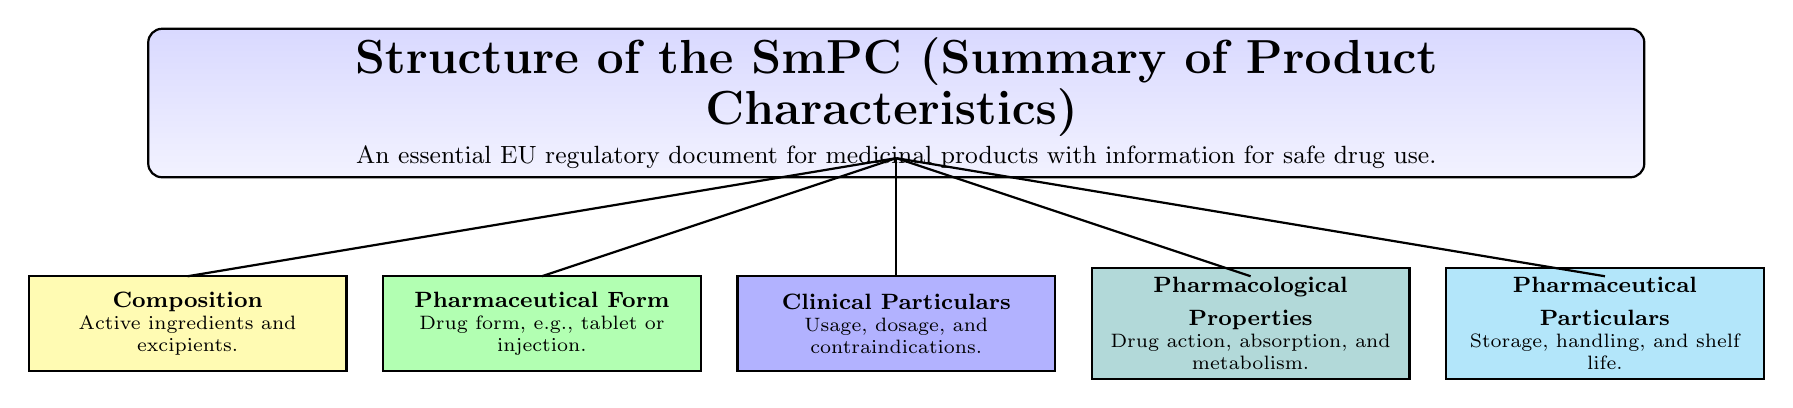
\begin{tikzpicture}
        % Title box with reduced height for a better fit
        \node[draw, thick, rounded corners=5pt, minimum width=19cm, minimum height=1.4cm, fill=blue!10!white, top color=blue!15, bottom color=blue!5] at (0, 2.8) {
            \begin{minipage}{17.5cm}
                \centering
                \textbf{\LARGE Structure of the SmPC (Summary of Product Characteristics)}
                \vspace{3pt}
                \small \\ An essential EU regulatory document for medicinal products with information for safe drug use.
            \end{minipage}
        };

        % Section boxes with exact positions
        % Composition box
        \node[draw, thick, fill=yellow!30, minimum width=3.8cm, minimum height=1.2cm] at (-9, 0) {
            \begin{minipage}{3.8cm}
                \centering
                \textbf{\footnotesize Composition} \\ 
                \scriptsize Active ingredients and excipients.
            \end{minipage}
        };
        
        % Pharmaceutical Form box
        \node[draw, thick, fill=green!30, minimum width=3.8cm, minimum height=1.2cm] at (-4.5, 0) {
            \begin{minipage}{3.8cm}
                \centering
                \textbf{\footnotesize Pharmaceutical Form} \\ 
                \scriptsize Drug form, e.g., tablet or injection.
            \end{minipage}
        };
        
        % Clinical Particulars box
        \node[draw, thick, fill=blue!30, minimum width=3.8cm, minimum height=1.2cm] at (0, 0) {
            \begin{minipage}{3.8cm}
                \centering
                \textbf{\footnotesize Clinical Particulars} \\ 
                \scriptsize Usage, dosage, and contraindications.
            \end{minipage}
        };
        
        % Pharmacological Properties box
        \node[draw, thick, fill=teal!30, minimum width=3.8cm, minimum height=1.2cm] at (4.5, 0) {
            \begin{minipage}{3.8cm}
                \centering
                \textbf{\footnotesize Pharmacological Properties} \\ 
                \scriptsize Drug action, absorption, and metabolism.
            \end{minipage}
        };
        
        % Pharmaceutical Particulars box
        \node[draw, thick, fill=cyan!30, minimum width=3.8cm, minimum height=1.2cm] at (9, 0) {
            \begin{minipage}{3.8cm}
                \centering
                \textbf{\footnotesize Pharmaceutical Particulars} \\ 
                \scriptsize Storage, handling, and shelf life.
            \end{minipage}
        };

        % Draw connecting lines with exact coordinates for alignment
        \draw[thick] (0, 2.1) -- (-9, 0.6);   % to Composition box
        \draw[thick] (0, 2.1) -- (-4.5, 0.6); % to Pharmaceutical Form box
        \draw[thick] (0, 2.1) -- (0, 0.6);    % to Clinical Particulars box
        \draw[thick] (0, 2.1) -- (4.5, 0.6);  % to Pharmacological Properties box
        \draw[thick] (0, 2.1) -- (9, 0.6);    % to Pharmaceutical Particulars box

    \end{tikzpicture}
    \end{adjustbox}
    \caption{Structure and Purpose of the SmPC (Summary of Product Characteristics)}
    \label{fig:smpc_structure}
\end{figure*}



Fine-tuning clinical LLM models involves adapting them to process clinical and biomedical texts effectively, as well as other types of medical data such as medical images, pathology reports, and diagnostic test results. This strategic approach enables the model to understand and generate insights from diverse data modalities, providing a more comprehensive understanding of patient information and enhancing the performance of healthcare-related tasks. 



\subsection{Large-scale Open Source Healthcare Datasets}
Table \ref{tab:open_source_dataset} provides descriptions for various open-source datasets related to healthcare and bioinformatics. The table presents descriptions for diverse datasets, encompassing aspects such as protein sequences, amino acids, antibodies, ncRNA sequences, compounds, patient data with chest X-ray images and radiology reports, and medical language processing tasks, offering a comprehensive overview of data in healthcare and bioinformatics.






\section{Leveraging Open LLMs for Prescription: A Case Study}
\label{sec:case_study}
This section presents a case study to investigate the prospects of using open LLMs in critical healthcare technologies, specifically for digitizing prescription analysis tasks. Our objective is to highlight the most relevant adverse drug reactions and interactions associated with prescribed medications based on a particular patient profile. Our motivation to focus is inspired by the work of Raza et al. \cite{raza2024generative}, which focuses on leveraging LLMs to enhance the accuracy of medication directions in pharmacy operations. While their work emphasizes ensuring the correct administration of medications, our study evaluates the suitability of the medication in the first place, i.e., determining which medicine product is relatively safer for a particular patient. Our investigation assesses the feasibility of using open LLMs for critical prescription tasks and compares their performance with proprietary counterparts. This case study also allows us to address the adaptation of open LLMs in accurately contextualizing complex patient and drug information for actionable insights guiding safe prescribing practices. Specifically, we aim to identify performance gaps and understand the viability of using open LLMs in complex healthcare contexts, we seek to answer the following pressing research questions:

\begin{quote}
\begin{itemize}
    \item[\textbf{RQ1}:] How effective are open LLMs in identifying adverse drug reactions compared to proprietary models?
    \item[\textbf{RQ2}:] What are the limitations and challenges of using open LLMs in prescription analysis?
    \item[\textbf{RQ3}:] How can the performance of open LLMs be made comparable to proprietary models, particularly by grounding them using techniques like Retrieval-Augmented Generation (RAG)?
\end{itemize}
\end{quote}

% \begin{itemize}
%     \item[RQ1:] Is it feasible to leverage open LLMs for developing critical clinical applications? 
%     \item[RQ2:] Does LLMs encode clinical knowledge and can they be used for information retrieval concerning clinical checks?  
%     \item[RQ3:] What are the limitations of open-source and closed-source LLMs in modeling clinical knowledge and how they can alleviated? 
% \end{itemize}

\subsection{Defining the Problem}
Safer prescribing practices are essential but increasingly challenging due to the vast amount of clinical guidance and patient-specific data that must be reviewed to make optimal decisions. Manual exploration of this information is impractical, given limited consultation times. LLMs offer a solution to this challenge. In this paper, we present a case study on using LLMs to enhance prescribing safety by assessing the suitability of medications for individual patients based on their Electronic Medical Record (EMR), referred to as the patient profile. EMRs capture diverse characteristics, including patient demographics, medical history such as allergies and diseases, past and present medications, laboratory results and vital signs, current diagnosis and symptoms, and surgical history. To assess adverse drug reactions (ADRs) and interactions at the point of prescribing, we prompt an LLM using a customized prompt encompassing the patient profile and the Summary of Product Characteristics (SmPC) for the given patient and medicine. The LLM is tasked with identifying medication suitability by highlighting various classes of interactions, including (1) Age; (2) Comorbidities; (3) Contraindications; (4) Dose; (5) Genetics; (6) Lactation; (7) Pregnancy; and (8) Warnings. The SmPC is an essential regulatory document used in Europe and United Kingdom for medicinal products that provides healthcare professionals with crucial information for the safe and effective administration of a drug. It serves as a comprehensive source of information, covering various aspects such as therapeutic indications, dosage, administration, contraindications, and side effects \cite{EU_SmPC}. SmPC is structured into six key sections as illustrated in Figure \ref{fig:smpc_structure}. This information should be reviewed in tandem with the patient's EMR to enable safer prescribing decisions and avoid ADRs.





% To assess the proficiency of LLaMA-2 in encoding clinical knowledge and evaluate its potential in the field of medicine, we turn to medical question answering. This undertaking poses a challenge as delivering high-quality responses to medical queries demands an understanding of medical context,,,, the recall of relevant medical knowledge, and the ability to reason with expert information \cite{singhal2022large}. 


% Our system features an interactive user interface that allows selecting predefined medications and patient profiles as well as adding customized patient profiles. The corresponding SmPC of the selected medication is automatically retrieved and displayed to the user, which is then supplemented in the prompts to LLMs to get personalized recommendations. All results are stored in the database and then manually validated by the clinical experts.


\subsection{Proposed Method for Prescription Evaluation}
To evaluate the proficiency of open and proprietary LLMs in encoding clinical knowledge and their potential for personalized prescriptions, we conducted a controlled experimental study. Specifically, we examined the effectiveness of various LLMs, including both open-source and closed-source models. As shown in Figure \ref{fig:method}, our proposed methodology consists of four major steps, including synthetic patient profile generation using GenAI, verification of generated patient profiles by expert clinicians, evaluating LLMs for prescription, and validating the results quantitatively and qualitatively. Below we provide a brief description of each step: 

\begin{figure*}[!t]
\centering
\includegraphics[width=\linewidth]{prescription_method.pdf}
\caption{Illustration of the proposed methodology for evaluating open and closed-source LLMs using two settings, i.e., with and without Retrieval Augmented Generation (RAG).}
\label{fig:method}
\end{figure*}   

\subsubsection{Data Description} 
The patient dataset used in this study was extracted from the public MIMIC-III (Medical Information Mart for Intensive Care) database \cite{mimiciii}, which contains de-identified health-related data from critical care patients. It contains de-identified health records from real patients providing rich clinical information, including patient demographics, diagnoses, medications, and treatment timelines. This dataset also provides valuable insights into the management of complex medical conditions, and this subset of data focuses on patients with chronic illnesses such as rheumatic heart disease, diabetes, and hypertension. Also, it includes detailed records of medications (e.g., Warfarin, Levothyroxine, Lisinopril, etc.), dosage, administration schedules, and as well as comorbidities like sepsis and heart failure. This allows for an in-depth analysis of drug administration patterns and clinical outcomes across a diverse patient population.

We leveraged the MIMIC-III dataset to create a set of 25 unique patient profiles that reflect real-world clinical scenarios while ensuring diversity in patient characteristics such as demographics, medical history, current medications, laboratory results, diagnoses, and symptoms. To make the profiles more personable, we assigned each patient a synthetic name to preserve anonymity, while ensuring the integrity of clinical data remained intact. The incorporation of synthetic names helps to humanize the profiles and provide a more relatable context for clinical scenarios. Each record includes a synthetic name and key patient characteristics such as age, gender, race, and blood type, along with primary diagnoses and comorbidities like sepsis, heart failure, and gastrointestinal disorders. The created patient profiles were formatted to a structured JSON format, which includes important characteristics such as patient demographics, diagnoses, medication history, and other key clinical details such as admission details, including the case's urgency (e.g., urgent, emergency, elective). Furthermore, it also contains comprehensive medication administration data, detailing the prescribed drugs (e.g., Warfarin, Levothyroxine, Lisinopril), their dosages, units, and administration schedules. Treatment courses are further described with start and end dates, indicating the duration and dosage adjustments for each medication. Our curated subset data provides a holistic view of patient management in cases of multi-morbidity, offering valuable insights into drug administration patterns, treatment efficacy, and clinical outcomes in a varied patient population.

\subsubsection{Verification of Patient Profiles} 
To ensure realism and clinical relevance, a team of expert clinicians reviewed and verified patient profiles created using the MIMIC-III dataset. If any inaccuracies or inconsistencies were identified among the various factors of a patient profile (e.g., demographics, diagnoses, or treatments), these were manually corrected to maintain the accuracy of the profiles. This verification process is a critical step in ensuring the validity of the experimental study and ensuring that the profiles accurately reflect real-world patient data. 

\begin{table*}[h!]
\centering
\caption{Medication Suitability Evaluation Prompt Template}
% \scriptsize
\begin{tabular}{p{17cm}}
\toprule
\textbf{Context}  \\
\midrule
You are an experienced and helpful prescribing assistant named Charlie. Charlie can support prescribers to carry out relevant checks when prescribing medication based on the patient medical profile and medical knowledge. You should tell us if the medication is suitable for the user based on the following patient profile and provide the result in JSON format: \\
\begin{quote}
\centering
$<$patient profile$>$
\end{quote} \\
\midrule
\textbf{Instructions} \\
\midrule
For each check, use the terms ``Suitable'' or ``Risky'' to indicate whether the medication is appropriate based on the given parameter. In overall suitability, the result should be given as a score. If any check is not relevant (such as pregnancy and lactation for males), mark it as N/A. \\
\midrule
\textbf{Output Format (JSON)}  \\
\midrule
\begin{verbatim}
{
  "Age": {"result": <result>, "reason": <reason>},
  "Dose": {"result": <result>, "reason": <reason>},
  "Comorbidities": {"result": <result>, "reason": <reason>},
  "Contraindications": {"result": <result>, "reason": <reason>},
  "Pregnancy": {"result": <result>, "reason": <reason>},
  "Lactation": {"result": <result>, "reason": <reason>},
  "Warnings": {"result": <result>, "reason": <reason>},
  "Genetics": {"result": <result>, "reason": <reason>},
  "Overall Suitability": {"score": <score>, "reason": <reason>}
}
\end{verbatim} \\
\bottomrule
\end{tabular}
\label{tab:prompt_template}
\end{table*}


\subsubsection{Evaluating LLMs for Prescription} We evaluate various open and closed-source LLMs for prescription tasks using the verified patient profiles and five different medications including Warfarin, Metformin, Levothyroxine, Lisinopril, and Omeprazole, for the analysis of each medication, we utilized their corresponding SmPC. The LLMs were tasked with identifying the suitability of the medications based on factors such as age, comorbidities, contraindications, dose, genetics, lactation, pregnancy, and warnings. Both open-source and proprietary models were evaluated to compare their performance in terms of accuracy and reliability in clinical decision-making. Furthermore, to improve the ability of LLMs to extract relevant information from SmPCs with greater precision, we utilized the Retrieval Augmented Generation (RAG) technique, which is widely recognized for addressing inherent LLM limitations such as hallucination \cite{ng2024rag}. It computes the Cosine distance between the input query and the vectorized SmPC document of the corresponding medication to retrieve the appropriate contextual information to generate accurate responses.

\subsubsection{Results Validation} The results generated by the LLMs were validated through a dual-validation approach that involves evaluating identified risks quantitatively using the ground truth information from the SmPC and qualitative assessment. We utilized various metrics, including accuracy, precision, recall, and F1-score, to quantify LLMs' performance. Qualitative validation involved detailed reviews by clinicians to assess the clinical soundness and practicality of the LLMs' recommendations. The medication to be prescribed is selected from a list of medicines in the database, which contains corresponding SmPC data. LLMs' responses detailing the ADR checks are formatted and stored in the database for each patient. We perform the subjective evaluation through an expert pharmacist possessing more than ten years of clinical experience. They assessed how well the LLMs identified ADRs and whether these identifications were consistent with the patient's medical histories, current diagnoses, and other relevant factors. Further details about the results will be provided in the next section.

\subsection{Results and Discussions}

\subsubsection{Experimental Setup and Implementation Details}
We evaluated the performance of five LLMs, including GPT-4, LLaMA-2, LLaMA-3, Mistral, and Meditron, for prescription tasks using a customized prompt template. These models are accessed through LangChain using the following chat models: ChatMistralAI, ChatOLLaMA (for LLaMA-2 and LLaMA-3), and ChatOpenAI. The Meditron model was deployed on Baseten(\url{https://docs.baseten.co/chains-reference/overview}) as a chat provider. We used default parameters for all models in our experiments. The SmPCs of the medications relevant to the experiment were parsed, cleaned, and vectorized. The vectorized SmPC documents were stored in a vector database, accessible for retrieval during the experiment. A consistent prompt was developed for each patient profile. The prompt contained the patient's information (age, gender, comorbidities, allergies, and current medications) and a question about the appropriateness of a prescription or a query regarding possible drug interactions, contraindications, or dosage adjustments. Table \ref{tab:prompt_template} describes the prompt template used for our analysis. The LangChain framework facilitated the interaction between the language model and the user query (prompt). It generated responses based on the LLM's understanding of the query and the knowledge retrieved by RAG. The RAG module employed the vectorized SmPC data to retrieve relevant sections of product information, which was then supplied to the LLM to enable fact-based response generation. The SmPC data was stored in a vector database to ensure rapid and efficient retrieval. A similarity-based search was executed using the query and patient profile to extract relevant details (e.g., dosing guidelines and drug interactions) from the SmPC vectors.






% This approach allowed us to systematically evaluate the effectiveness of the LLMs in encoding clinical knowledge and their utility in personalized prescriptions, while also validating their efficacy and utility in clinical settings.

% As described earlier, our experimental design involves querying LLMs while presenting patient profiles with and without SmPC information, recording the results, and collecting expert opinions for analysis. Patient profiles, particularly focusing on a case study of diabetes, were derived from the MIMIC III dataset \cite{johnson2016mimic}. An example patient profile can be seen in the Appendix \ref{tab:my-table}. We considered a zero-shot approach, assuming that the LLMs were not trained using \href{https://huggingface.co/datasets/sophy/smpc?row=0}{SmPC data}. To ensure a fair comparison, we utilized the same prompt template and information while evaluating the models above, incorporating SmPC information of a given medicine and the patient profile. The prompt template used for our analysis is described in the Appendix. \textcolor{blue}{For example, Table \ref{tab:prompt-template} illustrates a prompt template that assesses the suitability of prescribing ibuprofen to a pregnant female patient with rheumatoid arthritis by evaluating risks, contraindications, warnings, comorbidities, drug interactions, allergic reactions, alternatives, age and weight suitability, pregnancy, and lactation concerns, along with SNOMED CT codes for medications or conditions. Dosage checks and SmPC data for ibuprofen are also considered.} This approach allowed us to systematically evaluate the effectiveness of the LLMs in encoding clinical knowledge and their utility in personalized prescriptions, while also validating their efficacy and utility in clinical settings. We used LangChain, a JavaScript-based framework for building applications powered by LLMs. It enables the utilization of language models to generate text based on given textual prompts. We integrated the OpenAI GPT-3.5-turbo model and \textcolor{blue}{LLaMA-3} model into our LangChain chat model and generated text embeddings using OpenAI API for both the LLaMA-3 and GPT models. The configuration parameters for ChatGPT setup include setting the temperature to 0 and the maximum number of new tokens to 4096. For formulating prompts,\textcolor{blue}{we utilized the prompt template which is illustrated in Table \ref{tab:prompt-template} }. That specified the role of the AI as a prescribing assistant and allowed for dynamic insertion of questions. Additionally, we employed LLaMACPP for interfacing with LLaMA-2, enabling seamless integration with local hardware and ensuring state-of-the-art performance. We used Python programming language for our experimental evaluation. In the LLaMA-2 setup, the configuration parameters included setting the temperature to 1, the number of tokens to 512, and the context length as 2048.



\subsubsection{Quantitative Results}
The main results of our experimental study on LLM-empowered personalized prescriptions are presented in Table \ref{tab:results}. The table reports the results in terms of different performance metrics including accuracy, precision, recall, and F1-score for five different LLMs namely, GPT-4, LLaMA-2, LLaMA-3, Mistral, and Meditron. Moreover, the table provides a comparative analysis of all models in two settings, i.e., with and without augmenting LLMs' responses using RAG. Table \ref{tab:results} reveals that the GPT-4 model (a proprietary LLM) outperforms other open-source models in terms of different performance metrics. Moreover, it can be seen that open-source LLMs, such as LLaMA-3, can achieve remarkable performance levels comparable to proprietary models like OpenAI's GPT-4. When examining the results across various interaction classes, LLaMA-3 often matches or even surpasses OpenAI's GPT-4 model in terms of accuracy, precision, recall, and F1 score. For instance, in critical interaction types such as contraindications, genetics, lactation, and pregnancy, LLaMA-3 shows consistently high performance. Both models (i.e., GPT-4 and LLaMA-3) achieve a perfect score in genetics and pregnancy interactions, demonstrating that LLaMA-3 can perform exceptionally well in these categories. Additionally, LLaMA-3 maintains immersive performance in other interactions like age, comorbidities, and warnings, where its scores are very close to those of GPT-4. This highlights the potential of open-source LLMs to deliver high-quality results on par with proprietary models. 

\begin{table*}[!t]
\centering
\caption{Comparative Analysis of Prescription using different open and closed-source LLMs.}
% \scriptsize
\label{tab:results}
\scalebox{0.9}{
\begin{tabular}{clcccc|cccc}
\toprule
\multirow{2}{*}{\textbf{LLM}} &
  \multicolumn{1}{c}{\multirow{2}{*}{\textbf{Interaction Type}}} &
  \multicolumn{4}{c|}{\textbf{Results without using RAG}} &
  \multicolumn{4}{c}{\textbf{Results using RAG}} \\
 &
  \multicolumn{1}{c}{} &
  \textbf{Accuracy} &
  \textbf{Precision} &
  \textbf{Recall} &
  \textbf{F1 Score} &
  \textbf{Accuracy} &
  \textbf{Precision} &
  \textbf{Recall} &
  \textbf{F1 Score} \\ \toprule
\multirow{8}{*}{\textbf{LLaMA-2}} & Age               &   0.87   &   0.88   &   0.88   &   0.78   &   0.88   &  0.87    &   0.88   &   0.85   \\
                                   & Comorbidities     &  0.71    &  0.87    &  0.71    &  0.74    &  0.78    &  0.88    & 0.78     &     0.76 \\
                                   & Contraindications  &   0.52   &  0.47    &   0.52   &   0.52   &   0.90   &   0.92   &   0.91   &  0.91   \\
                                   % & Contraindications &   0.90   &   0.92   &   0.91   &  0.91    &   0.52   &  0.47    &   0.52   &   0.52   \\
                                   & Dose              &  0.68    &   0.68   &  0.68    &  0.68    &  0.71    &   0.73   &   0.71   &     0.70 \\
                                   & Genetics          &  0.88    &  0.88    &   0.88   &   0.88   &  0.96    &   0.95   &  0.94    &    0.95  \\
                                   & Lactation         &  1.00    &  1.00    &  1.00    &  1.00    &  0.63    &  0.98    &  0.63    &     0.66 \\
                                   & Pregnancy         &  1.00    &  1.00    &  1.00    &  1.00    &   0.84   &   0.70   &  0.84    &     0.76 \\
                                   & Warnings          &  0.70    &   0.81   &   0.70   &  0.75    &  0.71    &  0.83    &   0.71   &  0.75    \\ \midrule
\multirow{8}{*}{\textbf{LLaMA-3}}  & Age               & 0.85 & 0.72 & 0.85 & 0.78 & 0.88 & 0.89 & 0.88 & 0.84 \\
                                   & Comorbidities     & 0.72 & 0.88 & 0.72 & 0.75 & 0.80 & 0.90 & 0.80 & 0.82 \\
                                   & Contraindications & 0.48 & 0.48 & 0.48 & 0.48 & 0.92 & 0.93 & 0.92 & 0.92 \\
                                   & Dose              & 0.70 & 0.70 & 0.70 & 0.70 & 0.72 & 0.82 & 0.72 & 0.70 \\
                                   & Genetics          & 0.92 & 0.92 & 0.92 & 0.92 & 0.96 & 0.96 & 0.96 & 0.96 \\
                                   & Lactation         & 1.00 & 1.00 & 1.00 & 1.00 & 0.50 & 1.00 & 0.50 & 0.67 \\
                                   & Pregnancy         & 1.00 & 1.00 & 1.00 & 1.00 & 0.83 & 0.69 & 0.83 & 0.76 \\
                                   & Warnings          & 0.64 & 0.89 & 0.64 & 0.74 & 0.71 & 0.82 & 0.71 & 0.76 \\ \midrule
\multirow{8}{*}{\textbf{Mistral}}  & Age               & 0.88     & 0.90     & 0.88    &    0.85  & 0.88     &  0.95    &    0.91  &  0.93    \\
                                   & Comorbidities     & 0.72     &  0.63    & 0.72     &  0.67    & 0.80     & 1.00     & 0.50     & 0.67     \\
                                   & Contraindications &   0.73   &  0.82    & 0.73     &  0.71    & 0.68     & 0.91     &  0.65    & 0.76     \\
                                   & Dose              &  0.48    &  0.49    &  0.48    & 0.37     &  0.64    &  0.95    &    0.64  &  0.76    \\
                                   & Genetics          &  1.00    & 1.00     &  1.00    &  1.00    & 0.95     & 1.00     &  0.50    &  0.67    \\
                                   & Lactation         & 1.00     & 1.00     & 1.00     & 1.00     & 1.00     & 1.00     &  1.00    &   1.00   \\
                                   & Pregnancy         &  0.83    &  0.69    &  0.83    &  0.76    & 0.95     &  1.00    &  0.50    &  0.67    \\
                                   & Warnings          & 0.58     & 0.80     &  0.58    & 0.68     & 0.76      &  0.92    &  0.85    &  0.88    \\ \midrule
\multirow{8}{*}{\textbf{Meditron}} & Age               & 0.89     &   0.88   &  0.89    &  0.88    &  0.89    &  0.89    &   0.89   &  0.85    \\
                                   & Comorbidities     &  0.70    &   0.87   &   0.70  &   0.75   &  0.81    &   0.91   &  0.81    &    0.83  \\
                                   & Contraindications &  0.49    &  0.49    &   0.49   &  0.49 &  0.91    &  0.93    &   0.91   &   0.92    \\
                                   & Dose              &  0.72    &   0.71   &  0.71    &  0.69    &  0.73    &  0.73    &  0.73    &     0.73 \\
                                   & Genetics          &  0.93    &   0.92   &   0.93   &   0.92   &  0.97    &   0.97   &  0.97    &  0.97    \\
                                   & Lactation         &  0.78    &  0.96   &  0.78    &  0.68    &  0.80    &  0.82    &  0.80    &     0.90 \\
                                   & Pregnancy         & 1.00     &  1.00    &   1.00   &  1.00    &  1.00    &  1.00    &  1.00    &   1.00   \\
                                   & Warnings          &  0.70    &  0.83    &  0.70    &   0.75   & 0.72     &   0.83   &  0.72    &     0.77 \\ \midrule
\multirow{8}{*}{\textbf{GPT4}}     & Age               & 0.80 & 0.86 & 0.80 & 0.82 & 0.80 & 0.86 & 0.80 & 0.82 \\
                                   & Comorbidities     & 0.76 & 0.80 & 0.76 & 0.77 & 0.88 & 0.87 & 0.88 & 0.87 \\
                                   & Contraindications & 0.52 & 0.53 & 0.52 & 0.51 & 0.75 & 0.76 & 0.75 & 0.75 \\
                                   & Dose              & 0.48 & 0.49 & 0.48 & 0.37 & 0.72 & 0.72 & 0.72 & 0.72 \\
                                   & Genetics          & 1.00 & 1.00 & 1.00 & 1.00 & 1.00 & 1.00 & 1.00 & 1.00 \\
                                   & Lactation         & 0.50 & 1.00 & 0.50 & 0.67 & 1.00 & 1.00 & 1.00 & 1.00 \\
                                   & Pregnancy         & 0.83 & 0.69 & 0.83 & 0.76 & 1.00 & 1.00 & 1.00 & 1.00 \\
                                   & Warnings          & 0.79 & 0.94 & 0.79 & 0.84 & 0.71 & 0.87 & 0.71 & 0.77 \\
                                   \bottomrule
\end{tabular}}
\end{table*}


Grounding open-source models is crucial, particularly in high-stakes domains like healthcare, where incorrect information can have serious consequences. The comparison of model performance with and without RAG clearly illustrates this point. For both LLaMA-3 and OpenAI's GPT-4, incorporating RAG significantly enhances their performance across almost all interaction types in terms of different metrics such as accuracy, precision, recall, and F1 scores. For example, LLaMA-3's accuracy in handling age interactions improves from 0.85\% to 0.88\% with RAG, and similar improvements are observed in comorbidities, warnings, and other categories. This trend is also reflected in GPT-4's scores, where incorporating RAG leads to improvements across various interaction types. The stark contrast in performance metrics highlights the importance of grounding these models with relevant and reliable data. Without such grounding, even the most advanced models may fail to deliver the accuracy and reliability required in sensitive applications. This highlights the need for robust data augmentation techniques in deploying AI systems in critical fields such as healthcare.


\subsubsection{Qualitative Results}
To evaluate the clinical significance of the personalized prescription provided by LLMs, we performed a subjective assessment through an expert clinician with more than 10 years of clinical experience, particularly focusing on managing complex cases involving multi-morbidity and polypharmacy. This expert, also a paper co-author, has been actively involved in the project since its inception. Below, we describe our methodology for conducting subjective assessment through the human expert and the findings of this analysis.



\paragraph{Evaluation Strategy for Subjective Assessment}
For the subjective evaluation, we carefully selected 12 patient profiles from our dataset while ensuring they represent a broad spectrum of clinical scenarios ranging from straightforward cases to those involving complex medication interactions. In the interest of expert time, we only select 12 patient profiles to provide a fair and comprehensive performance evaluation of the LLM-driven prescription. The expert prescriber was asked to subjectively evaluate the efficacy of the AI-generated prescriptions by considering the following key clinical features:

\begin{itemize}
    \item \textit{Medication Selection Accuracy (MSA)}: How appropriate is the medication choice in the AI-generated prescription compared to traditional methods?
    \item \textit{Drug Interaction Detection (DID)}: How effectively does the AI system identify and mitigate potential drug interactions compared to the expert's judgment?
    \item \textit{Patient-Specific Dosage Adjustment (PSDA)}: How accurately does the AI system adjust dosages for special populations such as elderly patients or those with renal impairment?
    \item \textit{Prescription Safety Score (PSS)}: What is the overall safety profile of the AI-generated prescription compared to traditional prescribing methods?
\end{itemize}

In addition to evaluating the aforementioned critical features, the expert was also asked to provide a general assessment of the LLMs' overall effectiveness in generating safe and patient-centered prescriptions without focusing on any specific feature (i.e., MSA, DID, PSDA, and PSS). To quantify the subjective assessment, we leveraged five-scale grading, i.e., 5: Excellent; 4: Very Good; 3: Good; 2: Average; and 1: Poor. 

\begin{figure*} [!t]
    \centering
    \includegraphics[width=1\linewidth]{qualitative_results.png}
    \caption{Comparative analysis of the qualitative assessment scores across different metrics for each patient profile. Each subplot represents a specific metric, where the color intensity reflects the scores of different models with and without retrieval-augmented generation (RAG).}
    \label{fig:qual_results}
\end{figure*}


\paragraph{Results using Subjective Assessment}
The results for the subjective analysis are summarized in Figure \ref{fig:qual_results}. The impact of grounding LLMs with RAG is evident, as RAG-enabled models consistently outperform their non-RAG counterparts, particularly in tasks involving critical decisions regarding medication safety and drug interactions such as DID and PSS. This demonstrates that RAG enables LLMs to access relevant contextual information, thereby improving their precision in complex and safety-sensitive scenarios. For instance, LLaMA-2 (RAG) consistently performed well in DID, receiving a score of 5 in all but one profile, demonstrating ``Excellent'' performance in identifying drug interactions. PSDA score for LLaMA-2 (RAG) is 4, which indicates a ``Very Good'' performance in recommending dosages for special patient groups. LLaMA-2 (RAG) consistently achieved a score of 5 in PSS, indicating an ``Excellent`` performance in terms of safety. The GA rating of LLaMA-2 (RAG) is also consistently 5, reflecting that the model handled patient-centered prescriptions effectively with RAG. Mistral (RAG) showed ``Excellent'' performance in DID, scoring 5 across most profiles. It also performed excellently in PSDA, with a score of 5 in most of the profiles, and received a consistent score of 5 for PSS, indicating a high level of safety. Similar to LLaMA-2 (RAG), the GA for Mistral (RAG) is consistently 5, showing that it is highly effective in generating patient-centered prescriptions.

Meditron (RAG) also performed exceptionally well in DID, receiving a consistent score of 5 for drug interaction detection. It is also highly rated for PSDA, receiving scores of 4 and 5 for dosage adjustments. PSS achieved an ``Excellent'' score of 5 across most profiles, ensuring patient safety. The GA for Meditron (RAG) is predominantly rated 5, reflecting strong overall performance. For GPT-4, both RAG and non-RAG variants perform consistently well. For instance, it received a maximum score (i.e., 5) for DID, demonstrating excellent capability in managing potential drug risks. For the GPT-4 (RAG) model, PSDA is rated 5 across nearly all profiles, reflecting high accuracy in dosage adjustments for special populations. GPT-4 (RAG) also received a score of 5 for PSS, ensuring strong safety management across all profiles, and its GA is consistently rated 5, indicating reliable patient-centered prescription generation.

Across all RAG-enabled models, DID and PSS consistently receive high ratings. This indicates that LLMs with RAG excel at ensuring patient safety and managing potential drug interactions. We observed lightly more variability for PSDA and MSA but the expert's ratings remained predominantly ``Very Good'' or ``Excellent.'' GA consistently achieved high ratings (i.e., 5), indicating that LLMs effectively provided patient-centered recommendations, especially with the inclusion of RAG. The last subplot in Figure \ref{fig:qual_results} presents a holistic view of the overall performance summary for each model with and without RAG. This average summary demonstrates that RAG-enabled models consistently achieve higher average scores compared to their non-RAG counterparts. This highlights the cumulative benefit of RAG across diverse metrics. Notably, the open-source models, when equipped with RAG, demonstrated strong results, approaching the reliability of GPT-4 (closed-source) in an overall patient-centered prescription generation. Such a competitive performance of RAG-enabled open-source models highlights their value as accessible and customizable alternatives to proprietary solutions.




% Table \ref{tab:SmPC_results} presents the results of experiments conducted to evaluate the performance of open (LLaMA-2 Chat) and closed (ChatGPT) LLMs in personalized prescription tasks when supplemented with relevant SmPC information and local medication guidance alongside the patient profile. The table also includes remarks provided by clinical experts who assessed the outcomes generated by both models. We observe an improvement in the models' responses when they are supplemented with relevant SmPC data, with ChatGPT providing more detailed responses covering all important aspects asked in the prompt. Whereas, in comparison, open-source LLaMA-2 Chat did not provide any response to a few important questions. Despite both models offering some personalized recommendations based on the provided information (i.e., patient profile, SmPC, and local guidance), their outcomes were deemed unreliable and incorrect by clinical experts. This highlights the inherent limitations of current LLMs in encoding the clinical information from intricate contexts such as prescriptions, which necessitate the interpretation of patient data encompassing medical history, current medications, SmPC details, and local prescribing guidelines. The inability of these models to navigate complex information underscores the pressing need for the development of customized and task-specific LLMs capable of meeting the high demands of reliable and safe clinical decision-making. 

% \subsubsection{Discussions}
% Our experiments showed that each model provided valuable insights, with common themes of risk management in dosage, comorbidities, and contraindications, as well as the need for genetic considerations to optimize treatment outcomes. The expert's recommendations were largely in line with the AI-generated assessments, particularly regarding risk factors like sepsis and the need for dosage adjustments. Open-source models like LLaMA performed competently, particularly in identifying general risk factors like bleeding and sepsis-related complications. However, compared to closed-source (OpenAI), the risk assessments were slightly less detailed. The open-source models did not emphasize the need for genetic testing as much as OpenAI did, which could be a missed opportunity for optimizing Warfarin use in the case of some patients. With SmPC, both open-source and closed-source models improved their recommendations, particularly in handling drug interactions and providing specific advice regarding monitoring and dosage adjustments.

% The open-source model(OpenAI) excelled in providing detailed, risk-sensitive recommendations, particularly when RAG was used. Its ability to account for potential drug interactions, specific contraindications, and the suggestion of genetic testing to optimize dosage demonstrated a more comprehensive and cautious approach. The performance was especially strong in managing complex risk factors like sepsis. Closed-source models performed competently, particularly in assessing general risks and handling drug interactions, and did even better with RAG, but their analysis was less comprehensive compared to OpenAI. While they flagged relevant risks and made appropriate recommendations, the depth of analysis and personalization of advice was slightly lacking in comparison. The models did improve with SmPC integration, but the advice was more standard and not as nuanced. This could be managed by improving the models to provide an explanation of uncertainty, alternative options, handling of special populations, and perhaps integration with real-time lab data. Other beneficial ways to improve the open-source models include adding clinical guidelines, relevant pharmacogenomics data, enhanced drug interaction checks, clinical risk calculators such as HAS-BLED, and customized follow-up recommendations. 

% Our experimental evaluation of open-sourced and closed-source LLMs highlights their limitations in effectively extracting relevant information necessary for making personalized prescriptions. For instance, the clinical experts noted that neither of the models was able to effectively extract accurate information from the provided data to adequately highlight the risks and adverse reactions associated with the medications under consideration. This failure can be attributed to the lack of task-specific training, underscoring the necessity for the development of LLMs tailored to specific tasks. Since clinical applications like prescriptions have a life-critical nature, these models should be meticulously trained using relevant data to ensure the effectiveness and safety of their outcomes. Furthermore, there is an immense need for the integration of techniques such as retrieval augmentation generation to enhance the groundedness of the retrieved information from intricate clinical data comprising SmPC, patient records, and local prescription guidance, etc. In addition, the integration of attention mechanisms and multi-modal fusion techniques can enhance the LLM's ability to capture subtle nuances and correlations within the clinical data. The incorporation of such approaches can facilitate the extraction of more accurate and contextually relevant information, thereby improving the overall performance and reliability of LLMs in critical clinical decision-making processes like prescriptions. Moreover, the need for explainability in LLMs cannot be overstated, enhanced explainability mechanisms are essential for elucidating the reasoning behind the model's recommendations, thereby fostering trustworthiness and transparency in the decision-making process. The incorporation of explainability features in LLMs-empowered personalized prescription systems will empower clinicians to better understand and interpret the model's outputs, ultimately enhancing trust and acceptance within clinical practice.



% \begin{figure}
%     \centering
%     \includegraphics[width=0.5\linewidth]{qualitative_analysis.jpeg}
%     \caption{Caption}
%     \label{fig:enter-label}
% \end{figure}

% \begin{table}[!ht]
% \centering
% \caption{Qualitative results }
% \label{tab:subject}
% \scalebox{0.95}{
% \begin{tabular}{cccccc} 
% \toprule
% \textbf{Patient Profile} &
%   \textbf{MSA} &
%   \textbf{DID} &
%   \textbf{PSDA} &
%   \textbf{PSS} &
%   \textbf{GA} \\ \toprule
% Profile 1  & 4.0$\pm$0.5 & 4.5$\pm$0.4 & 3.8$\pm$0.6 & 4.2$\pm$0.5 & 4.5$\pm$0.4 \\
% Profile 2  & 4.2$\pm$0.4 & 4.3$\pm$0.5 & 4.0$\pm$0.4 & 4.3$\pm$0.4 & 4.5$\pm$0.5 \\
% Profile 3  & 3.8$\pm$0.6 & 4.0$\pm$0.5 & 3.5$\pm$0.7 & 4.1$\pm$0.5 & 4.2$\pm$0.5 \\
% Profile 4  & 4.1$\pm$0.4 & 4.4$\pm$0.4 & 3.9$\pm$0.5 & 4.3$\pm$0.4 & 4.6$\pm$0.4 \\
% Profile 5  & 3.9$\pm$0.5 & 4.2$\pm$0.5 & 3.6$\pm$0.6 & 4.0$\pm$0.5 & 4.3$\pm$0.4 \\
% Profile 6  & 4.0$\pm$0.5 & 4.3$\pm$0.4 & 3.8$\pm$0.5 & 4.2$\pm$0.4 & 4.4$\pm$0.4 \\
% Profile 7  & 4.3$\pm$0.3 & 4.5$\pm$0.4 & 4.1$\pm$0.4 & 4.4$\pm$0.4 & 4.6$\pm$0.3 \\
% Profile 8  & 3.7$\pm$0.6 & 4.1$\pm$0.5 & 3.6$\pm$0.7 & 4.0$\pm$0.5 & 4.2$\pm$0.5 \\
% Profile 9  & 4.2$\pm$0.4 & 4.3$\pm$0.5 & 4.0$\pm$0.4 & 4.3$\pm$0.4 & 4.5$\pm$0.4 \\
% Profile 10 & 4.1$\pm$0.5 & 4.2$\pm$0.4 & 3.9$\pm$0.5 & 4.2$\pm$0.5 & 4.4$\pm$0.5 \\
% Profile 11 & 3.9$\pm$0.5 & 4.1$\pm$0.5 & 3.7$\pm$0.6 & 4.0$\pm$0.5 & 4.3$\pm$0.4 \\
% Profile 12 & 4.0$\pm$0.5 & 4.3$\pm$0.4 & 3.8$\pm$0.5 & 4.2$\pm$0.4 & 4.5$\pm$0.4 \\ \bottomrule
% \end{tabular}}
% \end{table}

% \section{The limitations of the paper.}
% \textcolor{blue}{
% The study faces several limitations that could impact the validity and generalizability of the findings. Firstly, the quality and diversity of the training data used for the LLMs are critical; the study relies on models like ChatGPT and LLaMA-3, which may not have been trained on sufficiently comprehensive and diverse healthcare datasets. This limitation potentially compromises the accuracy and reliability of the model's outputs. Secondly, the generalizability of the results is restricted, as the findings may not apply universally across all patient populations or healthcare settings due to the specific conditions and datasets examined in this study.
% Moreover, the inherent black-box nature of LLMs poses a significant challenge. The lack of interpretability makes it difficult for clinicians to understand the decision-making process of the models, which can hinder clinical adoption and erode trust in the AI's recommendations. Additionally, handling patient data raises considerable privacy and security concerns, which might not be fully addressed within the scope of this study, posing risks to data protection.
% Finally, the integration of LLMs into clinical workflows and decision-making processes is crucial for their effectiveness in practice, yet this study might not fully explore how well these AI models align with and support human clinicians in real-world scenarios.
% These limitations underscore the need for ongoing research and development to enhance the application of LLMs in healthcare, ensuring they are trained on comprehensive datasets, are interpretable, integrate seamlessly with clinical workflows, and adhere to stringent regulatory and ethical standards.}


\section{Conclusions}
\label{sec:concs}
In this paper, we have made two major contributions. Firstly, we conduct a comprehensive survey and develop a detailed taxonomy of current developments and challenges in open-source Large Language Models (LLMs) and Artificial Intelligence Foundation Models (AIFMs). Secondly, we present a case study focused on LLMs-empowered personalized prescriptions, where the objective is to analyze the feasibility of using open LLMs for critical clinical tasks like prescriptions and compare their performance with closed-source models. Our exploration of open LLMs and AIFMs in healthcare highlights a pivotal shift towards more accessible and transparent AI technologies in healthcare, emphasizing the growing potential of open-source solutions. Our comprehensive survey and taxonomy provide a structured overview of the current landscape, identifying both the strengths and limitations of open-source LLMs and AIFMs within healthcare applications. The case study on personalized prescriptions demonstrates the practical capabilities of open-source LLMs in providing effective patient-centered recommendations. Our experimental findings reveal that open-source LLMs lag behind similar proprietary models, but their performance can be improved by equipping them with other technologies such as Retrieval Augmented Generation (RAG). Despite this performance gap, open-source LLMs and AIFMs are emerging as promising solutions for AI-empowered healthcare, particularly considering their adaptability, accessibility, and customization. While open-source LLMs and AIFMs present significant opportunities, the ethical concerns and risks of misuse cannot be overlooked. Therefore, we emphasize the need for ongoing research, responsible development, and rigorous governance in deploying these powerful tools in healthcare environments. 


\section*{Acknowledgment}
The authors would like to acknowledge support from the Qatar University High Impact Internal Grant (QUHI-CENG23/24-127). The statements made herein are solely the responsibility of the authors.


\bibliographystyle{IEEEtran}
% \bibliography{refs}

% Generated by IEEEtran.bst, version: 1.14 (2015/08/26)
\begin{thebibliography}{100}
\providecommand{\url}[1]{#1}
\csname url@samestyle\endcsname
\providecommand{\newblock}{\relax}
\providecommand{\bibinfo}[2]{#2}
\providecommand{\BIBentrySTDinterwordspacing}{\spaceskip=0pt\relax}
\providecommand{\BIBentryALTinterwordstretchfactor}{4}
\providecommand{\BIBentryALTinterwordspacing}{\spaceskip=\fontdimen2\font plus
\BIBentryALTinterwordstretchfactor\fontdimen3\font minus \fontdimen4\font\relax}
\providecommand{\BIBforeignlanguage}[2]{{%
\expandafter\ifx\csname l@#1\endcsname\relax
\typeout{** WARNING: IEEEtran.bst: No hyphenation pattern has been}%
\typeout{** loaded for the language `#1'. Using the pattern for}%
\typeout{** the default language instead.}%
\else
\language=\csname l@#1\endcsname
\fi
#2}}
\providecommand{\BIBdecl}{\relax}
\BIBdecl

\bibitem{wang2017heterogeneous}
L.~Wang, ``Heterogeneous data and big data analytics,'' \emph{Automatic Control and Information Sciences}, vol.~3, no.~1, pp. 8--15, 2017.

\bibitem{radford2019language}
A.~Radford, J.~Wu, R.~Child, D.~Luan, D.~Amodei, I.~Sutskever \emph{et~al.}, ``Language models are unsupervised multitask learners,'' \emph{OpenAI blog}, vol.~1, no.~8, p.~9, 2019.

\bibitem{mann2020language}
B.~Mann, N.~Ryder, M.~Subbiah, J.~Kaplan, P.~Dhariwal, A.~Neelakantan, P.~Shyam, G.~Sastry, A.~Askell, S.~Agarwal \emph{et~al.}, ``Language models are few-shot learners,'' \emph{arXiv preprint arXiv:2005.14165}, 2020.

\bibitem{fedus2022switch}
W.~Fedus, B.~Zoph, and N.~Shazeer, ``Switch transformers: Scaling to trillion parameter models with simple and efficient sparsity,'' \emph{The Journal of Machine Learning Research}, vol.~23, no.~1, pp. 5232--5270, 2022.

\bibitem{bubeck2023sparks}
S.~Bubeck, V.~Chandrasekaran, R.~Eldan, J.~Gehrke, E.~Horvitz, E.~Kamar, P.~Lee, Y.~T. Lee, Y.~Li, S.~Lundberg \emph{et~al.}, ``Sparks of artificial general intelligence: Early experiments with {GPT}-4,'' \emph{arXiv preprint arXiv:2303.12712}, 2023.

\bibitem{wang2018glue}
A.~Wang, A.~Singh, J.~Michael, F.~Hill, O.~Levy, and S.~R. Bowman, ``{GLUE}: A multi-task benchmark and analysis platform for natural language understanding,'' \emph{arXiv preprint arXiv:1804.07461}, 2018.

\bibitem{sakaguchi2021winogrande}
K.~Sakaguchi, R.~L. Bras, C.~Bhagavatula, and Y.~Choi, ``Winogrande: An adversarial winograd schema challenge at scale,'' \emph{Communications of the ACM}, vol.~64, no.~9, pp. 99--106, 2021.

\bibitem{brown2020language}
T.~Brown, B.~Mann, N.~Ryder, M.~Subbiah, J.~D. Kaplan, P.~Dhariwal, A.~Neelakantan, P.~Shyam, G.~Sastry, A.~Askell \emph{et~al.}, ``Language models are few-shot learners,'' \emph{Advances in neural information processing systems}, vol.~33, pp. 1877--1901, 2020.

\bibitem{wornow2024zero}
``Zero-shot clinical trial patient matching with {LLMs}.''

\bibitem{chen2020recall}
S.~Chen, Y.~Hou, Y.~Cui, W.~Che, T.~Liu, and X.~Yu, ``Recall and learn: Fine-tuning deep pretrained language models with less forgetting,'' \emph{arXiv preprint arXiv:2004.12651}, 2020.

\bibitem{chua2021fine}
K.~Chua, Q.~Lei, and J.~D. Lee, ``How fine-tuning allows for effective meta-learning,'' \emph{Advances in Neural Information Processing Systems}, vol.~34, pp. 8871--8884, 2021.

\bibitem{ju2022robust}
H.~Ju, D.~Li, and H.~R. Zhang, ``Robust fine-tuning of deep neural networks with hessian-based generalization guarantees,'' in \emph{International Conference on Machine Learning}.\hskip 1em plus 0.5em minus 0.4em\relax PMLR, 2022, pp. 10\,431--10\,461.

\bibitem{vulic2021lexfit}
I.~Vuli{\'c}, E.~M. Ponti, A.~Korhonen, and G.~Glava{\v{s}}, ``Lexfit: Lexical fine-tuning of pretrained language models,'' in \emph{Proceedings of the 59th Annual Meeting of the Association for Computational Linguistics and the 11th International Joint Conference on Natural Language Processing (Volume 1: Long Papers)}, 2021, pp. 5269--5283.

\bibitem{zhang2020revisiting}
T.~Zhang, F.~Wu, A.~Katiyar, K.~Q. Weinberger, and Y.~Artzi, ``Revisiting few-sample {BERT} fine-tuning,'' \emph{arXiv preprint arXiv:2006.05987}, 2020.

\bibitem{seger2023open}
E.~Seger, N.~Dreksler, R.~Moulange, E.~Dardaman, J.~Schuett, K.~Wei, C.~Winter, M.~Arnold, S.~{\'O}. h{\'E}igeartaigh, A.~Korinek \emph{et~al.}, ``Open-sourcing highly capable foundation models: An evaluation of risks, benefits, and alternative methods for pursuing open-source objectives,'' \emph{arXiv preprint arXiv:2311.09227}, 2023.

\bibitem{kapoorposition}
S.~Kapoor, R.~Bommasani, K.~Klyman, S.~Longpre, A.~Ramaswami, P.~Cihon, A.~K. Hopkins, K.~Bankston, S.~Biderman, M.~Bogen \emph{et~al.}, ``Position paper: On the societal impact of open foundation models,'' in \emph{Forty-first International Conference on Machine Learning}.

\bibitem{thieme2023foundation}
A.~Thieme, A.~Nori, M.~Ghassemi, R.~Bommasani, T.~O. Andersen, and E.~Luger, ``Foundation models in healthcare: Opportunities, risks \& strategies forward,'' in \emph{Extended Abstracts of the 2023 CHI Conference on Human Factors in Computing Systems}, 2023, pp. 1--4.

\bibitem{vaswani2017attention}
A.~Vaswani, N.~Shazeer, N.~Parmar, J.~Uszkoreit, L.~Jones, A.~N. Gomez, {\L}.~Kaiser, and I.~Polosukhin, ``Attention is all you need,'' \emph{Advances in neural information processing systems}, vol.~30, 2017.

\bibitem{he2023survey}
K.~He, R.~Mao, Q.~Lin, Y.~Ruan, X.~Lan, M.~Feng, and E.~Cambria, ``A survey of large language models for healthcare: from data, technology, and applications to accountability and ethics,'' \emph{arXiv preprint arXiv:2310.05694}, 2023.

\bibitem{bommasani2021opportunities}
R.~Bommasani, D.~A. Hudson, E.~Adeli, R.~Altman, S.~Arora, S.~von Arx, M.~S. Bernstein, J.~Bohg, A.~Bosselut, E.~Brunskill \emph{et~al.}, ``On the opportunities and risks of foundation models,'' \emph{arXiv preprint arXiv:2108.07258}, 2021.

\bibitem{solaiman2023gradient}
I.~Solaiman, ``The gradient of generative {AI} release: Methods and considerations,'' in \emph{Proceedings of the 2023 ACM Conference on Fairness, Accountability, and Transparency}, 2023, pp. 111--122.

\bibitem{roziere2023code}
B.~Roziere, J.~Gehring, F.~Gloeckle, S.~Sootla, I.~Gat, X.~E. Tan, Y.~Adi, J.~Liu, T.~Remez, J.~Rapin \emph{et~al.}, ``Code llama: Open foundation models for code,'' \emph{arXiv preprint arXiv:2308.12950}, 2023.

\bibitem{carugati2023competition}
C.~Carugati, ``Competition in generative artificial intelligence foundation models,'' Bruegel Working Paper, Tech. Rep., 2023.

\bibitem{gurrieri2023d2}
M.~Gurrieri, E.~Daga, A.~Scharnhorst, and J.~Carvalho, ``D2. 6: Ontology of licencing, ownership and conditions of use (v1. 0),'' Ph.D. dissertation, Open University, 2023.

\bibitem{alizadeh2023open}
M.~Alizadeh, M.~Kubli, Z.~Samei, S.~Dehghani, J.~D. Bermeo, M.~Korobeynikova, and F.~Gilardi, ``Open-source large language models outperform crowd workers and approach {ChatGPT} in text-annotation tasks,'' \emph{arXiv preprint arXiv:2307.02179}, 2023.

\bibitem{osi1998definition}
\BIBentryALTinterwordspacing
{Open Source Initiative}, ``The open source definition (osd),'' 1998, accessed: 2024-12-01. [Online]. Available: \url{https://opensource.org/history}
\BIBentrySTDinterwordspacing

\bibitem{dibona1999open}
C.~DiBona and S.~Ockman, \emph{Open sources: Voices from the open source revolution}.\hskip 1em plus 0.5em minus 0.4em\relax " O'Reilly Media, Inc.", 1999.

\bibitem{touvron2023LLaMA}
H.~Touvron, L.~Martin, K.~Stone, P.~Albert, A.~Almahairi, Y.~Babaei, N.~Bashlykov, S.~Batra, P.~Bhargava, S.~Bhosale \emph{et~al.}, ``Llama 2: Open foundation and fine-tuned chat models,'' \emph{arXiv preprint arXiv:2307.09288}, 2023.

\bibitem{kapoor2024societal}
S.~Kapoor, R.~Bommasani, K.~Klyman, S.~Longpre, A.~Ramaswami, P.~Cihon, A.~Hopkins, K.~Bankston, S.~Biderman, M.~Bogen \emph{et~al.}, ``On the societal impact of open foundation models,'' 2024.

\bibitem{spector2023accelerating}
B.~Spector and C.~Re, ``Accelerating {LLM} inference with staged speculative decoding,'' \emph{arXiv preprint arXiv:2308.04623}, 2023.

\bibitem{khalid2023privacy}
N.~Khalid, A.~Qayyum, M.~Bilal, A.~Al-Fuqaha, and J.~Qadir, ``Privacy-preserving artificial intelligence in healthcare: Techniques and applications,'' \emph{Computers in Biology and Medicine}, p. 106848, 2023.

\bibitem{inan2021training}
H.~A. Inan, O.~Ramadan, L.~Wutschitz, D.~Jones, V.~R{\"u}hle, J.~Withers, and R.~Sim, ``Training data leakage analysis in language models,'' \emph{arXiv preprint arXiv:2101.05405}, 2021.

\bibitem{carlini2021extracting}
N.~Carlini, F.~Tramer, E.~Wallace, M.~Jagielski, A.~Herbert-Voss, K.~Lee, A.~Roberts, T.~Brown, D.~Song, U.~Erlingsson \emph{et~al.}, ``Extracting training data from large language models,'' in \emph{30th USENIX Security Symposium (USENIX Security 21)}, 2021, pp. 2633--2650.

\bibitem{torkzadehmahani2022privacy}
R.~Torkzadehmahani, R.~Nasirigerdeh, D.~B. Blumenthal, T.~Kacprowski, M.~List, J.~Matschinske, J.~Spaeth, N.~K. Wenke, and J.~Baumbach, ``Privacy-preserving artificial intelligence techniques in biomedicine,'' \emph{Methods of Information in Medicine}, vol.~61, pp. e12--e27, 2022.

\bibitem{zou2020privacy}
Y.~Zou, Z.~Zhang, M.~Backes, and Y.~Zhang, ``Privacy analysis of deep learning in the wild: Membership inference attacks against transfer learning,'' \emph{arXiv preprint arXiv:2009.04872}, 2020.

\bibitem{pan2020privacy}
X.~Pan, M.~Zhang, S.~Ji, and M.~Yang, ``Privacy risks of general-purpose language models,'' in \emph{2020 IEEE Symposium on Security and Privacy (SP)}.\hskip 1em plus 0.5em minus 0.4em\relax IEEE, 2020, pp. 1314--1331.

\bibitem{goldstein2023generative}
J.~A. Goldstein, G.~Sastry, M.~Musser, R.~DiResta, M.~Gentzel, and K.~Sedova, ``Generative language models and automated influence operations: Emerging threats and potential mitigations,'' \emph{arXiv preprint arXiv:2301.04246}, 2023.

\bibitem{bender2021dangers}
E.~M. Bender, T.~Gebru, A.~McMillan-Major, and S.~Shmitchell, ``On the dangers of stochastic parrots: Can language models be too big?'' in \emph{Proceedings of the 2021 ACM conference on fairness, accountability, and transparency}, 2021, pp. 610--623.

\bibitem{zhou2021machine}
Q.~Zhou, M.~Zuley, Y.~Guo, L.~Yang, B.~Nair, A.~Vargo, S.~Ghannam, D.~Arefan, and S.~Wu, ``A machine and human reader study on {AI} diagnosis model safety under attacks of adversarial images,'' \emph{Nature communications}, vol.~12, no.~1, p. 7281, 2021.

\bibitem{qayyum2020secure}
A.~Qayyum, J.~Qadir, M.~Bilal, and A.~Al-Fuqaha, ``Secure and robust machine learning for healthcare: A survey,'' \emph{IEEE Reviews in Biomedical Engineering}, vol.~14, pp. 156--180, 2020.

\bibitem{finlayson2018adversarial}
S.~G. Finlayson, H.~W. Chung, I.~S. Kohane, and A.~L. Beam, ``Adversarial attacks against medical deep learning systems,'' \emph{arXiv preprint arXiv:1804.05296}, 2018.

\bibitem{finlayson2019adversarial}
S.~G. Finlayson, J.~D. Bowers, J.~Ito, J.~L. Zittrain, A.~L. Beam, and I.~S. Kohane, ``Adversarial attacks on medical machine learning,'' \emph{Science}, vol. 363, no. 6433, pp. 1287--1289, 2019.

\bibitem{paschali2018generalizability}
M.~Paschali, S.~Conjeti, F.~Navarro, and N.~Navab, ``Generalizability vs. robustness: adversarial examples for medical imaging,'' \emph{arXiv preprint arXiv:1804.00504}, 2018.

\bibitem{han2020deep}
X.~Han, Y.~Hu, L.~Foschini, L.~Chinitz, L.~Jankelson, and R.~Ranganath, ``Deep learning models for electrocardiograms are susceptible to adversarial attack,'' \emph{Nature medicine}, vol.~26, no.~3, pp. 360--363, 2020.

\bibitem{wang2023ethical}
C.~Wang, S.~Liu, H.~Yang, J.~Guo, Y.~Wu, and J.~Liu, ``Ethical considerations of using {ChatGPT} in health care,'' \emph{Journal of Medical Internet Research}, vol.~25, p. e48009, 2023.

\bibitem{john2024re}
J.-M. John-Mathews, R.~De~Mourat, D.~Ricci, and M.~Cr{\'e}pel, ``Re-enacting machine learning practices to enquire into the moral issues they pose,'' \emph{Convergence}, vol.~30, no.~1, pp. 66--93, 2024.

\bibitem{oakley2023hipaa}
A.~Oakley, ``{HIPAA, HIPPA, or HIPPO}: What really is the heath insurance portability and accountability act?'' \emph{Biotechnology Law Report}, 2023.

\bibitem{carmi2023european}
L.~Carmi, M.~Zohar, and G.~M. Riva, ``The european general data protection regulation ({GDPR}) in mhealth: Theoretical and practical aspects for practitioners’ use,'' \emph{Medicine, Science and the Law}, vol.~63, no.~1, pp. 61--68, 2023.

\bibitem{wei2022chain}
J.~Wei, X.~Wang, D.~Schuurmans, M.~Bosma, F.~Xia, E.~Chi, Q.~V. Le, D.~Zhou \emph{et~al.}, ``Chain-of-thought prompting elicits reasoning in large language models,'' \emph{Advances in Neural Information Processing Systems}, vol.~35, pp. 24\,824--24\,837, 2022.

\bibitem{singhal2022large}
K.~Singhal, S.~Azizi, T.~Tu, S.~S. Mahdavi, J.~Wei, H.~W. Chung, N.~Scales, A.~Tanwani, H.~Cole-Lewis, S.~Pfohl \emph{et~al.}, ``Large language models encode clinical knowledge,'' \emph{arXiv preprint arXiv:2212.13138}, 2022.

\bibitem{radford2021learning}
A.~Radford, J.~W. Kim, C.~Hallacy, A.~Ramesh, G.~Goh, S.~Agarwal, G.~Sastry, A.~Askell, P.~Mishkin, J.~Clark \emph{et~al.}, ``Learning transferable visual models from natural language supervision,'' in \emph{International conference on machine learning}.\hskip 1em plus 0.5em minus 0.4em\relax PMLR, 2021, pp. 8748--8763.

\bibitem{qiu2023visionfm}
J.~Qiu, J.~Wu, H.~Wei, P.~Shi, M.~Zhang, Y.~Sun, L.~Li, H.~Liu, H.~Liu, S.~Hou \emph{et~al.}, ``Visionfm: a multi-modal multi-task vision foundation model for generalist ophthalmic artificial intelligence,'' \emph{arXiv preprint arXiv:2310.04992}, 2023.

\bibitem{zhou2023foundation}
Y.~Zhou, M.~A. Chia, S.~K. Wagner, M.~S. Ayhan, D.~J. Williamson, R.~R. Struyven, T.~Liu, M.~Xu, M.~G. Lozano, P.~Woodward-Court \emph{et~al.}, ``A foundation model for generalizable disease detection from retinal images,'' \emph{Nature}, vol. 622, no. 7981, pp. 156--163, 2023.

\bibitem{mh2024lvm}
D.~MH~Nguyen, H.~Nguyen, N.~Diep, T.~N. Pham, T.~Cao, B.~Nguyen, P.~Swoboda, N.~Ho, S.~Albarqouni, P.~Xie \emph{et~al.}, ``Lvm-med: Learning large-scale self-supervised vision models for medical imaging via second-order graph matching,'' \emph{Advances in Neural Information Processing Systems}, vol.~36, 2024.

\bibitem{lehmann2023gloria}
M.~K. Lehmann, D.~Gurlin, N.~Pahlevan, K.~Alikas, T.~Conroy, J.~Anstee, S.~V. Balasubramanian, C.~C. Barbosa, C.~Binding, A.~Bracher \emph{et~al.}, ``{GLORIA-A} globally representative hyperspectral in situ dataset for optical sensing of water quality,'' \emph{Scientific Data}, vol.~10, no.~1, p. 100, 2023.

\bibitem{yin2023lamm}
Z.~Yin, J.~Wang, J.~Cao, Z.~Shi, D.~Liu, M.~Li, L.~Sheng, L.~Bai, X.~Huang, Z.~Wang \emph{et~al.}, ``{LAMM}: Language-assisted multi-modal instruction-tuning dataset, framework, and benchmark,'' \emph{arXiv preprint arXiv:2306.06687}, 2023.

\bibitem{zuo2023plip}
J.~Zuo, C.~Yu, N.~Sang, and C.~Gao, ``{PLIP}: Language-image pre-training for person representation learning,'' \emph{arXiv preprint arXiv:2305.08386}, 2023.

\bibitem{praveen2023understanding}
S.~Praveen and V.~Vajrobol, ``Understanding the perceptions of healthcare researchers regarding {ChatGPT}: a study based on bidirectional encoder representation from transformers ({BERT}) sentiment analysis and topic modeling,'' \emph{Annals of Biomedical Engineering}, pp. 1--3, 2023.

\bibitem{sharaf2023analysis}
S.~Sharaf and V.~Anoop, ``An analysis on large language models in healthcare: A case study of {BioBERT},'' \emph{arXiv preprint arXiv:2310.07282}, 2023.

\bibitem{vaishya2023chatgpt}
R.~Vaishya, A.~Misra, and A.~Vaish, ``{ChatGPT}: Is this version good for healthcare and research?'' \emph{Diabetes \& Metabolic Syndrome: Clinical Research \& Reviews}, vol.~17, no.~4, p. 102744, 2023.

\bibitem{clusmann2023future}
J.~Clusmann, F.~R. Kolbinger, H.~S. Muti, Z.~I. Carrero, J.-N. Eckardt, N.~G. Laleh, C.~M.~L. L{\"o}ffler, S.-C. Schwarzkopf, M.~Unger, G.~P. Veldhuizen \emph{et~al.}, ``The future landscape of large language models in medicine,'' \emph{Communications Medicine}, vol.~3, no.~1, p. 141, 2023.

\bibitem{wornow2023shaky}
M.~Wornow, Y.~Xu, R.~Thapa, B.~Patel, E.~Steinberg, S.~Fleming, M.~A. Pfeffer, J.~Fries, and N.~H. Shah, ``The shaky foundations of large language models and foundation models for electronic health records,'' \emph{npj Digital Medicine}, vol.~6, no.~1, p. 135, 2023.

\bibitem{wang2023anypredict}
Z.~Wang, C.~Gao, C.~Xiao, and J.~Sun, ``{AnyPredict: Foundation Model for Tabular Prediction},'' \emph{arXiv preprint arXiv:2305.12081}, 2023.

\bibitem{guo2023ehr}
L.~L. Guo, E.~Steinberg, S.~L. Fleming, J.~Posada, J.~Lemmon, S.~R. Pfohl, N.~Shah, J.~Fries, and L.~Sung, ``Ehr foundation models improve robustness in the presence of temporal distribution shift,'' \emph{Scientific Reports}, vol.~13, no.~1, p. 3767, 2023.

\bibitem{singhal2023large}
K.~Singhal, S.~Azizi, T.~Tu, S.~S. Mahdavi, J.~Wei, H.~W. Chung, N.~Scales, A.~Tanwani, H.~Cole-Lewis, S.~Pfohl \emph{et~al.}, ``Large language models encode clinical knowledge,'' \emph{Nature}, vol. 620, no. 7972, pp. 172--180, 2023.

\bibitem{liu2023deid}
Z.~Liu, X.~Yu, L.~Zhang, Z.~Wu, C.~Cao, H.~Dai, L.~Zhao, W.~Liu, D.~Shen, Q.~Li \emph{et~al.}, ``{DeID-GPT: zero-shot medical text de-identification by GPT-4},'' \emph{arXiv}, 2023.

\bibitem{waisberg2023gpt}
E.~Waisberg, J.~Ong, M.~Masalkhi, S.~A. Kamran, N.~Zaman, P.~Sarker, A.~G. Lee, and A.~Tavakkoli, ``{GPT-4}: a new era of artificial intelligence in medicine,'' \emph{Irish Journal of Medical Science (1971-)}, pp. 1--4, 2023.

\bibitem{ali2023chatgpt}
H.~Ali, J.~Qadir, and Z.~Shah, ``{ChatGPT and Large Language Models (LLMs) in Healthcare: Opportunities and Risks},'' 2023.

\bibitem{gu2021domain}
Y.~Gu, R.~Tinn, H.~Cheng, M.~Lucas, N.~Usuyama, X.~Liu, T.~Naumann, J.~Gao, and H.~Poon, ``Domain-specific language model pretraining for biomedical natural language processing,'' \emph{ACM Transactions on Computing for Healthcare (HEALTH)}, vol.~3, no.~1, pp. 1--23, 2021.

\bibitem{sun2023pathasst}
Y.~Sun, C.~Zhu, S.~Zheng, K.~Zhang, Z.~Shui, X.~Yu, Y.~Zhao, H.~Li, Y.~Zhang, R.~Zhao \emph{et~al.}, ``{PathAsst: Redefining Pathology through Generative Foundation {AI} Assistant for Pathology},'' \emph{arXiv preprint arXiv:2305.15072}, 2023.

\bibitem{balas2023conversational}
M.~Balas and E.~B. Ing, ``{Conversational {AI} models for ophthalmic diagnosis: Comparison of {ChatGPT} and the Isabel pro differential diagnosis generator},'' \emph{JFO Open Ophthalmology}, vol.~1, p. 100005, 2023.

\bibitem{levine2023diagnostic}
D.~M. Levine, R.~Tuwani, B.~Kompa, A.~Varma, S.~G. Finlayson, A.~Mehrotra, and A.~Beam, ``The diagnostic and triage accuracy of the {GPT-3} artificial intelligence model,'' \emph{medRxiv}, pp. 2023--01, 2023.

\bibitem{xie2023faithful}
Q.~Xie, E.~J. Schenck, H.~S. Yang, Y.~Chen, Y.~Peng, and F.~Wang, ``{Faithful {AI} in Medicine: A Systematic Review with Large Language Models and Beyond},'' \emph{Medrxiv: the Preprint Server for Health Sciences}, 2023.

\bibitem{biswas2023chatgpt}
S.~Biswas, ``{ChatGPT and the future of medical writing},'' p. e223312, 2023.

\bibitem{deng2023segment}
R.~Deng, C.~Cui, Q.~Liu, T.~Yao, L.~W. Remedios, S.~Bao, B.~A. Landman, L.~E. Wheless, L.~A. Coburn, K.~T. Wilson \emph{et~al.}, ``{Segment Anything Model (SAM) for Digital Pathology: Assess Zero-shot Segmentation on Whole Slide Imaging},'' \emph{arXiv preprint arXiv:2304.04155}, 2023.

\bibitem{putz2023segment}
F.~Putz, J.~Grigo, T.~Weissmann, P.~Schubert, D.~Hoefler, A.~Gomaa, H.~B. Tkhayat, A.~Hagag, S.~Lettmaier, B.~Frey \emph{et~al.}, ``The segment anything foundation model achieves favorable brain tumor autosegmentation accuracy on {MRI} to support radiotherapy treatment planning,'' \emph{arXiv preprint arXiv:2304.07875}, 2023.

\bibitem{zhao2023clinical}
X.~Zhao, J.-W. Bai, Q.~Guo, K.~Ren, and G.-J. Zhang, ``Clinical applications of deep learning in breast {MRI},'' \emph{Biochimica et Biophysica Acta (BBA)-Reviews on Cancer}, p. 188864, 2023.

\bibitem{chen2023pancreatic}
P.-T. Chen, T.~Wu, P.~Wang, D.~Chang, K.-L. Liu, M.-S. Wu, H.~R. Roth, P.-C. Lee, W.-C. Liao, and W.~Wang, ``Pancreatic cancer detection on {CT} scans with deep learning: a nationwide population-based study,'' \emph{Radiology}, vol. 306, no.~1, pp. 172--182, 2023.

\bibitem{nori2023capabilities}
H.~Nori, N.~King, S.~M. McKinney, D.~Carignan, and E.~Horvitz, ``Capabilities of {GPT-4} on medical challenge problems,'' \emph{arXiv preprint arXiv:2303.13375}, 2023.

\bibitem{li2023artificial}
X.~Li, L.~Zhang, Z.~Wu, Z.~Liu, L.~Zhao, Y.~Yuan, J.~Liu, G.~Li, D.~Zhu, P.~Yan \emph{et~al.}, ``Artificial general intelligence for medical imaging,'' \emph{arXiv preprint arXiv:2306.05480}, 2023.

\bibitem{zhang2023challenges}
S.~Zhang and D.~Metaxas, ``On the challenges and perspectives of foundation models for medical image analysis,'' \emph{arXiv preprint arXiv:2306.05705}, 2023.

\bibitem{shi2023generalist}
P.~Shi, J.~Qiu, S.~M.~D. Abaxi, H.~Wei, F.~P.-W. Lo, and W.~Yuan, ``Generalist vision foundation models for medical imaging: A case study of segment anything model on zero-shot medical segmentation,'' \emph{Diagnostics}, vol.~13, no.~11, p. 1947, 2023.

\bibitem{ji2304segment}
W.~Ji, J.~Li, Q.~Bi, W.~Li, and L.~Cheng, ``Segment anything is not always perfect: An investigation of sam on different real-world applications. arxiv 2023,'' \emph{arXiv preprint arXiv:2304.05750}.

\bibitem{dash2023evaluation}
D.~Dash, R.~Thapa, J.~M. Banda, A.~Swaminathan, M.~Cheatham, M.~Kashyap, N.~Kotecha, J.~H. Chen, S.~Gombar, L.~Downing \emph{et~al.}, ``Evaluation of {GPT-3.5 and GPT-4} for supporting real-world information needs in healthcare delivery,'' \emph{arXiv preprint arXiv:2304.13714}, 2023.

\bibitem{eggmann2023implications}
F.~Eggmann, R.~Weiger, N.~U. Zitzmann, and M.~B. Blatz, ``Implications of large language models such as {ChatGPT} for dental medicine,'' \emph{Journal of Esthetic and Restorative Dentistry}, 2023.

\bibitem{eysenbach2023role}
G.~Eysenbach \emph{et~al.}, ``The role of {ChatGPT}, generative language models, and artificial intelligence in medical education: a conversation with {ChatGPT} and a call for papers,'' \emph{JMIR Medical Education}, vol.~9, no.~1, p. e46885, 2023.

\bibitem{kung2023performance}
T.~H. Kung, M.~Cheatham, A.~Medenilla, C.~Sillos, L.~De~Leon, C.~Elepa{\~n}o, M.~Madriaga, R.~Aggabao, G.~Diaz-Candido, J.~Maningo \emph{et~al.}, ``{Performance of {ChatGPT} on USMLE: Potential for AI-assisted medical education using large language models},'' \emph{PLoS digital health}, vol.~2, no.~2, p. e0000198, 2023.

\bibitem{van2023if}
L.~Van~Bulck and P.~Moons, ``What if your patient switches from dr. google to dr. {ChatGPT}? a vignette-based survey of the trustworthiness, value, and danger of {ChatGPT}-generated responses to health questions,'' \emph{European Journal of Cardiovascular Nursing}, p. zvad038, 2023.

\bibitem{fraiwan2023review}
M.~Fraiwan and N.~Khasawneh, ``A review of {ChatGPT} applications in education, marketing, software engineering, and healthcare: Benefits, drawbacks, and research directions,'' \emph{arXiv preprint arXiv:2305.00237}, 2023.

\bibitem{abd2023large}
A.~Abd-Alrazaq, R.~AlSaad, D.~Alhuwail, A.~Ahmed, P.~M. Healy, S.~Latifi, S.~Aziz, R.~Damseh, S.~A. Alrazak, J.~Sheikh \emph{et~al.}, ``Large language models in medical education: Opportunities, challenges, and future directions,'' \emph{JMIR Medical Education}, vol.~9, no.~1, p. e48291, 2023.

\bibitem{teebagy2023improved}
S.~Teebagy, L.~Colwell, E.~Wood, A.~Yaghy, and M.~Faustina, ``Improved performance of {ChatGPT-4 on the OKAP} exam: A comparative study with {ChatGPT}-3.5,'' \emph{medRxiv}, pp. 2023--04, 2023.

\bibitem{antaki2023evaluating}
F.~Antaki, S.~Touma, D.~Milad, J.~El-Khoury, and R.~Duval, ``Evaluating the performance of {ChatGPT} in ophthalmology: An analysis of its successes and shortcomings,'' \emph{Ophthalmology Science}, p. 100324, 2023.

\bibitem{gill2023chatgpt}
S.~S. Gill and R.~Kaur, ``{ChatGPT: Vision and challenges},'' \emph{Internet of Things and Cyber-Physical Systems}, vol.~3, pp. 262--271, 2023.

\bibitem{kjell2023ai}
O.~Kjell, K.~Kjell, and H.~A. Schwartz, ``{AI-}based large language models are ready to transform psychological health assessment,'' 2023.

\bibitem{li2023chatgpt}
J.~Li, A.~Dada, J.~Kleesiek, and J.~Egger, ``{ChatGPT} in healthcare: A taxonomy and systematic review,'' \emph{medRxiv}, pp. 2023--03, 2023.

\bibitem{ray2023chatgpt}
P.~P. Ray, ``{ChatGPT}: A comprehensive review on background, applications, key challenges, bias, ethics, limitations and future scope,'' \emph{Internet of Things and Cyber-Physical Systems}, 2023.

\bibitem{yunxiang2023chatdoctor}
L.~Yunxiang, L.~Zihan, Z.~Kai, D.~Ruilong, and Z.~You, ``Chatdoctor: A medical chat model fine-tuned on llama model using medical domain knowledge,'' \emph{arXiv preprint arXiv:2303.14070}, 2023.

\bibitem{li2023chatdoctor}
Y.~Li, Z.~Li, K.~Zhang, R.~Dan, S.~Jiang, and Y.~Zhang, ``Chatdoctor: A medical chat model fine-tuned on a large language model meta-ai (llama) using medical domain knowledge,'' \emph{Cureus}, vol.~15, no.~6, 2023.

\bibitem{wu2023pmc}
C.~Wu, X.~Zhang, Y.~Zhang, Y.~Wang, and W.~Xie, ``Pmc-llama: Further finetuning llama on medical papers,'' \emph{arXiv preprint arXiv:2304.14454}, 2023.

\bibitem{haupt2023ai}
C.~E. Haupt and M.~Marks, ``{AI}-generated medical advice---{GPT} and beyond,'' \emph{Jama}, vol. 329, no.~16, pp. 1349--1350, 2023.

\bibitem{javaid2023chatgpt}
M.~Javaid, A.~Haleem, and R.~P. Singh, ``{ChatGPT} for healthcare services: An emerging stage for an innovative perspective,'' \emph{BenchCouncil Transactions on Benchmarks, Standards and Evaluations}, vol.~3, no.~1, p. 100105, 2023.

\bibitem{johnson2023assessing}
D.~Johnson, R.~Goodman, J.~Patrinely, C.~Stone, E.~Zimmerman, R.~Donald, S.~Chang, S.~Berkowitz, A.~Finn, E.~Jahangir \emph{et~al.}, ``Assessing the accuracy and reliability of {AI-}generated medical responses: an evaluation of the chat-gpt model,'' 2023.

\bibitem{moons2023chatgpt}
P.~Moons and L.~Van~Bulck, ``{ChatGPT}: can artificial intelligence language models be of value for cardiovascular nurses and allied health professionals,'' \emph{European journal of cardiovascular nursing}, 2023.

\bibitem{iftikhar2023docgpt}
L.~Iftikhar \emph{et~al.}, ``{DocGPT}: Impact of {ChatGPT}-3 on health services as a virtual doctor,'' \emph{EC Paediatrics}, vol.~12, no.~1, pp. 45--55, 2023.

\bibitem{ide2023can}
K.~Ide, P.~Hawke, and T.~Nakayama, ``Can {ChatGPT} be considered an author of a medical article?'' \emph{Journal of Epidemiology}, p. JE20230030, 2023.

\bibitem{muftic2023exploring}
F.~Mufti{\'c}, M.~Kaduni{\'c}, A.~Mu{\v{s}}inbegovi{\'c}, and A.~Abd~Almisreb, ``Exploring medical breakthroughs: A systematic review of {ChatGPT} applications in healthcare,'' \emph{Southeast Europe Journal of Soft Computing}, vol.~12, no.~1, pp. 13--41, 2023.

\bibitem{de2023chatgpt}
L.~De~Angelis, F.~Baglivo, G.~Arzilli, G.~P. Privitera, P.~Ferragina, A.~E. Tozzi, and C.~Rizzo, ``{ChatGPT and the rise of large language models: the new AI-driven infodemic threat in public health},'' \emph{Frontiers in Public Health}, vol.~11, p. 1166120, 2023.

\bibitem{snoswell2023artificial}
C.~L. Snoswell, A.~J. Snoswell, J.~T. Kelly, L.~J. Caffery, and A.~C. Smith, ``Artificial intelligence: Augmenting telehealth with large language models,'' \emph{Journal of telemedicine and telecare}, p. 1357633X231169055, 2023.

\bibitem{ahmed2024deep}
F.~A. Ahmed, M.~Yousef, M.~A. Ahmed, H.~O. Ali, A.~Mahboob, H.~Ali, Z.~Shah, O.~Aboumarzouk, A.~A. Ansari, and S.~Balakrishnan, ``Deep learning for surgical instrument recognition and segmentation in robotic-assisted surgeries: A systematic review,'' \emph{arXiv preprint arXiv:2410.07269}, 2024.

\bibitem{nori2023can}
H.~Nori, Y.~T. Lee, S.~Zhang, D.~Carignan, R.~Edgar, N.~Fusi, N.~King, J.~Larson, Y.~Li, W.~Liu \emph{et~al.}, ``Can generalist foundation models outcompete special-purpose tuning? case study in medicine,'' \emph{arXiv preprint arXiv:2311.16452}, 2023.

\bibitem{abi2023large}
J.~Abi-Rafeh, H.~H. Xu, R.~Kazan, R.~Tevlin, and H.~Furnas, ``Large language models and artificial intelligence: A primer for plastic surgeons on the demonstrated \& potential applications, promises, and limitations of {ChatGPT},'' \emph{Aesthetic Surgery Journal}, p. sjad260, 2023.

\bibitem{lee2020biobert}
J.~Lee, W.~Yoon, S.~Kim, D.~Kim, S.~Kim, C.~H. So, and J.~Kang, ``Biobert: a pre-trained biomedical language representation model for biomedical text mining,'' \emph{Bioinformatics}, vol.~36, no.~4, pp. 1234--1240, 2020.

\bibitem{shin2020biomegatron}
H.-C. Shin, Y.~Zhang, E.~Bakhturina, R.~Puri, M.~Patwary, M.~Shoeybi, and R.~Mani, ``Biomegatron: Larger biomedical domain language model,'' \emph{arXiv preprint arXiv:2010.06060}, 2020.

\bibitem{rasmy2021med}
L.~Rasmy, Y.~Xiang, Z.~Xie, C.~Tao, and D.~Zhi, ``Med-bert: pretrained contextualized embeddings on large-scale structured electronic health records for disease prediction,'' \emph{NPJ digital medicine}, vol.~4, no.~1, p.~86, 2021.

\bibitem{raj2021bioelectra}
K.~raj Kanakarajan, B.~Kundumani, and M.~Sankarasubbu, ``Bioelectra: pretrained biomedical text encoder using discriminators,'' in \emph{Proceedings of the 20th Workshop on Biomedical Language Processing}, 2021, pp. 143--154.

\bibitem{yuan2021improving}
Z.~Yuan, Y.~Liu, C.~Tan, S.~Huang, and F.~Huang, ``Improving biomedical pretrained language models with knowledge,'' \emph{arXiv preprint arXiv:2104.10344}, 2021.

\bibitem{lu2022clinicalt5}
Q.~Lu, D.~Dou, and T.~Nguyen, ``Clinicalt5: A generative language model for clinical text,'' in \emph{Findings of the Association for Computational Linguistics: EMNLP 2022}, 2022, pp. 5436--5443.

\bibitem{yasunaga2022linkbert}
M.~Yasunaga, J.~Leskovec, and P.~Liang, ``Linkbert: Pretraining language models with document links,'' \emph{arXiv preprint arXiv:2203.15827}, 2022.

\bibitem{luo2022biogpt}
R.~Luo, L.~Sun, Y.~Xia, T.~Qin, S.~Zhang, H.~Poon, and T.-Y. Liu, ``{BioGPT}: generative pre-trained transformer for biomedical text generation and mining,'' \emph{Briefings in Bioinformatics}, vol.~23, no.~6, p. bbac409, 2022.

\bibitem{yan2022radbert}
A.~Yan, J.~McAuley, X.~Lu, J.~Du, E.~Y. Chang, A.~Gentili, and C.-N. Hsu, ``{RadBERT}: Adapting transformer-based language models to radiology,'' \emph{Radiology: Artificial Intelligence}, vol.~4, no.~4, p. e210258, 2022.

\bibitem{cheng2022fastfold}
S.~Cheng, X.~Zhao, G.~Lu, J.~Fang, Z.~Yu, T.~Zheng, R.~Wu, X.~Zhang, J.~Peng, and Y.~You, ``Fastfold: Reducing alphafold training time from 11 days to 67 hours,'' \emph{arXiv preprint arXiv:2203.00854}, 2022.

\bibitem{yang2023enhancing}
J.~Yang, C.~Liu, W.~Deng, D.~Wu, C.~Weng, Y.~Zhou, and K.~Wang, ``Enhancing phenotype recognition in clinical notes using large language models: Phenobcbert and phenogpt,'' \emph{Patterns}, 2023.

\bibitem{wang2023chatcad}
S.~Wang, Z.~Zhao, X.~Ouyang, Q.~Wang, and D.~Shen, ``Chatcad: Interactive computer-aided diagnosis on medical image using large language models,'' \emph{arXiv preprint arXiv:2302.07257}, 2023.

\bibitem{shoham2023cpllm}
O.~B. Shoham and N.~Rappoport, ``Cpllm: Clinical prediction with large language models,'' \emph{arXiv preprint arXiv:2309.11295}, 2023.

\bibitem{xiong2023doctorglm}
H.~Xiong, S.~Wang, Y.~Zhu, Z.~Zhao, Y.~Liu, Q.~Wang, and D.~Shen, ``Doctorglm: Fine-tuning your chinese doctor is not a herculean task,'' \emph{arXiv preprint arXiv:2304.01097}, 2023.

\bibitem{singhal2023towards}
K.~Singhal, T.~Tu, J.~Gottweis, R.~Sayres, E.~Wulczyn, L.~Hou, K.~Clark, S.~Pfohl, H.~Cole-Lewis, D.~Neal \emph{et~al.}, ``Towards expert-level medical question answering with large language models,'' \emph{arXiv preprint arXiv:2305.09617}, 2023.

\bibitem{yang2022gatortron}
X.~Yang, N.~PourNejatian, H.~C. Shin, K.~E. Smith, C.~Parisien, C.~Compas, C.~Martin, M.~G. Flores, Y.~Zhang, T.~Magoc \emph{et~al.}, ``Gatortron: A large language model for clinical natural language processing,'' \emph{medRxiv}, pp. 2022--02, 2022.

\bibitem{zhang2023huatuogpt}
H.~Zhang, J.~Chen, F.~Jiang, F.~Yu, Z.~Chen, J.~Li, G.~Chen, X.~Wu, Z.~Zhang, Q.~Xiao \emph{et~al.}, ``{HuatuoGPT, towards Taming Language Model to Be a Doctor},'' \emph{arXiv preprint arXiv:2305.15075}, 2023.

\bibitem{chen2024dragonfly}
K.~Chen, R.~Thapa, R.~Chalamala, B.~Athiwaratkun, S.~L. Song, and J.~Zou, ``Dragonfly: Multi-resolution zoom supercharges large visual-language model,'' \emph{arXiv preprint arXiv:2406.00977}, 2024.

\bibitem{blankemeier2024merlin}
L.~Blankemeier, J.~P. Cohen, A.~Kumar, D.~Van~Veen, S.~J.~S. Gardezi, M.~Paschali, Z.~Chen, J.-B. Delbrouck, E.~Reis, C.~Truyts \emph{et~al.}, ``Merlin: A vision language foundation model for 3d computed tomography,'' \emph{arXiv preprint arXiv:2406.06512}, 2024.

\bibitem{team2024chameleon}
C.~Team, ``Chameleon: Mixed-modal early-fusion foundation models,'' \emph{arXiv preprint arXiv:2405.09818}, 2024.

\bibitem{chen2023meditron}
Z.~Chen, A.~H. Cano, A.~Romanou, A.~Bonnet, K.~Matoba, F.~Salvi, M.~Pagliardini, S.~Fan, A.~K{\"o}pf, A.~Mohtashami \emph{et~al.}, ``Meditron-70b: Scaling medical pretraining for large language models,'' \emph{arXiv preprint arXiv:2311.16079}, 2023.

\bibitem{srivastav2024maira}
S.~Srivastav, M.~Ranjit, F.~P{\'e}rez-Garc{\'\i}a, K.~Bouzid, S.~Bannur, D.~C. Castro, A.~Schwaighofer, H.~Sharma, M.~Ilse, V.~Salvatelli \emph{et~al.}, ``Maira at rrg24: A specialised large multimodal model for radiology report generation,'' in \emph{Proceedings of the 23rd Workshop on Biomedical Natural Language Processing}, 2024, pp. 597--602.

\bibitem{han2023medalpaca}
T.~Han, L.~C. Adams, J.-M. Papaioannou, P.~Grundmann, T.~Oberhauser, A.~L{\"o}ser, D.~Truhn, and K.~K. Bressem, ``{MedAlpaca--An Open-Source Collection of Medical Conversational {AI} Models and Training Data},'' \emph{arXiv preprint arXiv:2304.08247}, 2023.

\bibitem{rando2023universal}
J.~Rando and F.~Tram{\`e}r, ``Universal jailbreak backdoors from poisoned human feedback,'' \emph{arXiv preprint arXiv:2311.14455}, 2023.

\bibitem{291199}
\BIBentryALTinterwordspacing
N.~Carlini, J.~Hayes, M.~Nasr, M.~Jagielski, V.~Sehwag, F.~Tram{\`e}r, B.~Balle, D.~Ippolito, and E.~Wallace, ``Extracting training data from diffusion models,'' in \emph{32nd USENIX Security Symposium (USENIX Security 23)}.\hskip 1em plus 0.5em minus 0.4em\relax Anaheim, CA: USENIX Association, Aug. 2023, pp. 5253--5270. [Online]. Available: \url{https://www.usenix.org/conference/usenixsecurity23/presentation/carlini}
\BIBentrySTDinterwordspacing

\bibitem{dai2023safe}
J.~Dai, X.~Pan, R.~Sun, J.~Ji, X.~Xu, M.~Liu, Y.~Wang, and Y.~Yang, ``Safe {RLHF}: Safe reinforcement learning from human feedback,'' \emph{arXiv preprint arXiv:2310.12773}, 2023.

\bibitem{kim2023towards}
S.~Kim, S.~Jung, B.~Kim, M.~Choi, J.~Shin, and J.~Lee, ``Towards safe self-distillation of internet-scale text-to-image diffusion models,'' \emph{arXiv preprint arXiv:2307.05977}, 2023.

\bibitem{raza2024generative}
M.~M. Raza, K.~P. Venkatesh, and J.~C. Kvedar, ``Generative {AI} and large language models in health care: pathways to implementation,'' \emph{npj Digital Medicine}, vol.~7, no.~1, p.~62, 2024.

\bibitem{EU_SmPC}
\BIBentryALTinterwordspacing
E.~M. Agency, ``Guideline on summary of product characteristics,'' \emph{Official Journal of the European Union}, 2009. [Online]. Available: \url{https://ec.europa.eu/health/sites/default/files/files/eudralex/vol-2/c/smpc_guideline_rev2_en.pdf}
\BIBentrySTDinterwordspacing

\bibitem{mimiciii}
\BIBentryALTinterwordspacing
A.~E. Johnson, T.~J. Pollard, L.~Shen, L.-w.~H. Lehman, M.~Feng, M.~Ghassemi, and R.~G. Mark, ``Mimic-iii, a freely accessible critical care database,'' \emph{Scientific Data}, vol.~3, p. 160035, 2016. [Online]. Available: \url{https://doi.org/10.1038/sdata.2016.35}
\BIBentrySTDinterwordspacing

\bibitem{ng2024rag}
K.~K.~Y. Ng, I.~Matsuba, and P.~C. Zhang, ``Rag in health care: A novel framework for improving communication and decision-making by addressing llm limitations,'' \emph{NEJM AI}, p. AIra2400380, 2024.

\end{thebibliography}





\end{document}



